% Guía completa de finnet. Compilar desde docs/latex/guia:
%   latexmk -lualatex guia.tex
\documentclass[11pt,a4paper,oneside]{book}

\usepackage{fontspec}
\usepackage[spanish,es-noshorthands,es-tabla,es-nodecimaldot]{babel}
\usepackage{amsmath,amssymb}
\setmainfont{TeX Gyre Pagella}
\setsansfont{TeX Gyre Heros}
\setmonofont{DejaVu Sans Mono}[Scale=0.82]
\usepackage[margin=2.4cm,headheight=14pt]{geometry}
\usepackage{graphicx}
\usepackage{booktabs,tabularx,longtable,array}
\usepackage{xcolor}
\usepackage[most]{tcolorbox}
\usepackage{fvextra}
\usepackage{enumitem}
\usepackage{tikz}
\usetikzlibrary{arrows.meta,positioning,shapes.geometric,fit,calc}
\usepackage{caption}
\usepackage{fancyhdr}
\usepackage{titlesec}
\usepackage[hidelinks]{hyperref}

\graphicspath{{../figuras/}{../../../figures/}}

\definecolor{azul}{HTML}{2563A8}
\definecolor{rojo}{HTML}{C2362B}
\definecolor{verde}{HTML}{2F7D5B}
\definecolor{ambar}{HTML}{E0A100}
\definecolor{gris}{HTML}{5F6B77}
\definecolor{fondo}{HTML}{F4F6F8}

\titleformat{\chapter}[display]{\sffamily\bfseries\huge\color{azul}}
  {\large\chaptertitlename\ \thechapter}{8pt}{}
\titleformat{\section}{\sffamily\bfseries\Large}{\thesection}{0.8em}{}
\titleformat{\subsection}{\sffamily\bfseries\large}{\thesubsection}{0.8em}{}
\titlespacing*{\chapter}{0pt}{-20pt}{24pt}

\pagestyle{fancy}
\fancyhf{}
\fancyhead[L]{\small\sffamily\color{gris}finnet · guía completa}
\fancyhead[R]{\small\sffamily\color{gris}\leftmark}
\fancyfoot[C]{\small\thepage}
\renewcommand{\headrulewidth}{0.3pt}

\setlength{\parskip}{0.45em}
\setlength{\parindent}{0pt}
\setlist{itemsep=0.2em,topsep=0.3em}
\captionsetup{font=small,labelfont=bf}

% Recuadros
\newtcolorbox{idea}[1][Intuición]{colback=azul!6,colframe=azul,fonttitle=\sffamily\bfseries,
  title=#1,boxrule=0.6pt,arc=2pt,left=6pt,right=6pt}
\newtcolorbox{nota}[1][Nota]{colback=ambar!8,colframe=ambar!80!black,fonttitle=\sffamily\bfseries,
  title=#1,boxrule=0.6pt,arc=2pt,left=6pt,right=6pt}
\newtcolorbox{clave}[1][Resultado clave]{colback=verde!7,colframe=verde,fonttitle=\sffamily\bfseries,
  title=#1,boxrule=0.6pt,arc=2pt,left=6pt,right=6pt}
\newtcolorbox{limite}[1][Límite honesto]{colback=rojo!6,colframe=rojo,fonttitle=\sffamily\bfseries,
  title=#1,boxrule=0.6pt,arc=2pt,left=6pt,right=6pt}

% Código: bloques monoespaciados con marco y título (archivo de origen)
\DefineVerbatimEnvironment{codigo}{Verbatim}{fontsize=\small,frame=single,
  framerule=0.4pt,rulecolor=\color{gris!50},framesep=3mm,breaklines=true,
  breakanywhere=true,labelposition=topline}
\newcommand{\archivo}[1]{\texttt{\color{azul}#1}}
\newcommand{\term}[1]{\textbf{#1}}

\hypersetup{pdftitle={finnet: guía completa},pdfauthor={Juan Diego Martínez Ayala}}

\begin{document}

\begin{titlepage}
\centering
\vspace*{2.5cm}
{\sffamily\bfseries\Huge\color{azul} finnet\par}
\vspace{0.6cm}
{\sffamily\LARGE Redes complejas, sincronización y riesgo\\[2pt] en sistemas de pagos digitales\par}
\vspace{0.8cm}
{\large Guía completa del proyecto: la idea, la base desde cero,\\ los resultados y el montaje del software\par}
\vspace{1.6cm}
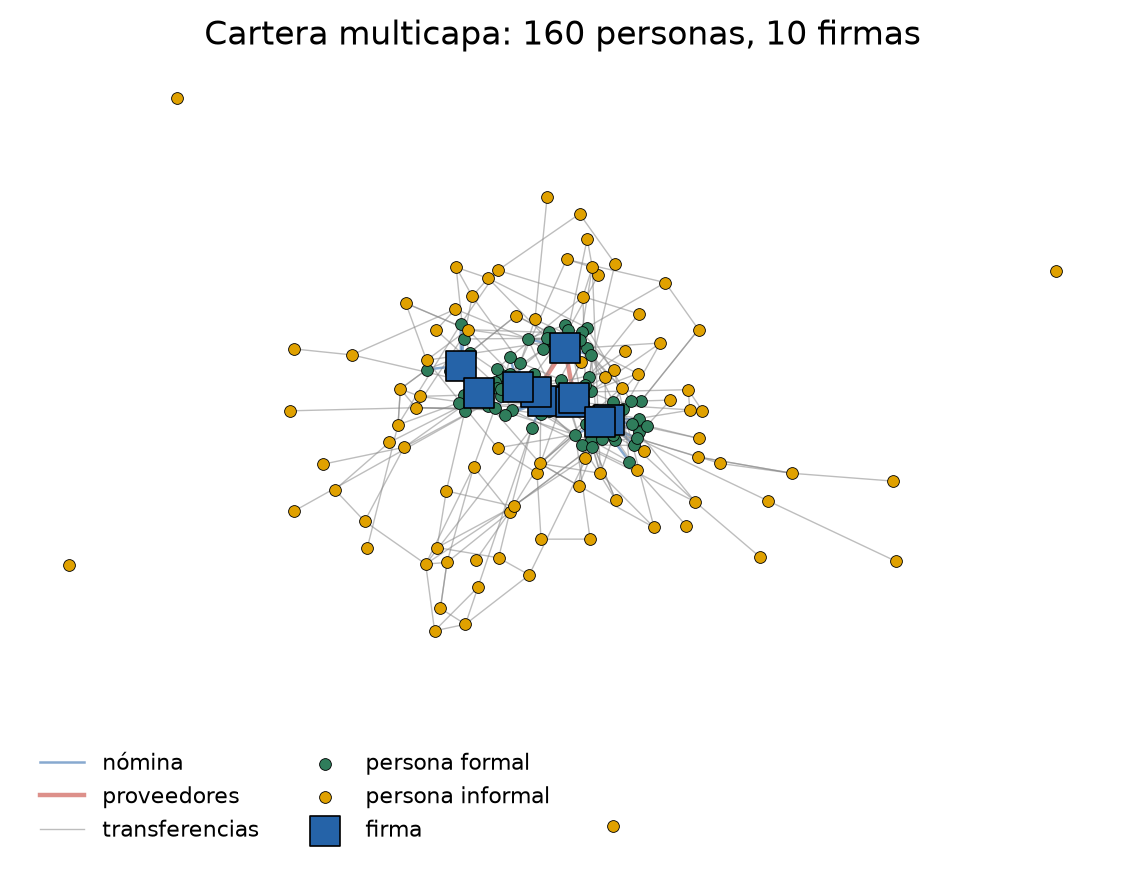
\includegraphics[width=0.78\textwidth]{tarea6_red_multicapa.png}\par
\vfill
{\large Juan Diego Martínez Ayala\par}
{\normalsize Dirección: Jhon Hernán Díaz Forero\par}
{\normalsize Semillero de Modelamiento de Sistemas Complejos y Física Computacional\par}
\vspace{0.4cm}
{\normalsize Versión del software 2.0.0 · noviembre de 2026\par}
\end{titlepage}

\frontmatter
\chapter*{Cómo leer esta guía}
\addcontentsline{toc}{chapter}{Cómo leer esta guía}
Esta guía está escrita para alguien que no conoce el tema: ni finanzas, ni redes,
ni el código. Cada concepto se explica la primera vez que aparece y se resume en el
glosario del final (apéndice~\ref{ap:glosario}).

\begin{itemize}
\item \textbf{Parte I · La idea} (capítulos 1–4). Qué problema se estudia, por qué
importa y cómo funciona el proyecto, sin ecuaciones. Si solo tiene veinte minutos,
lea esta parte.
\item \textbf{Parte II · La base desde cero} (capítulos 5–12). Cada pieza del modelo,
de la matemática mínima al código que la implementa, en el orden en que se
construyó (las seis tareas de la propuesta del semillero) y cómo se unen.
\item \textbf{Parte III · Resultados} (capítulos 13–15). Qué se verificó, qué se
encontró y qué \emph{no} se puede concluir.
\item \textbf{Parte IV · Montaje del software} (capítulos 16–19). Las herramientas,
cómo instalar y correr todo, un recorrido por la aplicación web y la organización
de las carpetas.
\end{itemize}

Convenciones visuales:
\begin{idea}[Intuición] Explicación con una analogía antes de la matemática.\end{idea}
\begin{nota}[Nota] Detalle técnico o decisión de diseño.\end{nota}
\begin{clave}[Resultado clave] Hallazgo principal de una sección.\end{clave}
\begin{limite}[Límite honesto] Lo que el resultado no demuestra.\end{limite}
Los nombres de archivo del proyecto aparecen así: \archivo{src/finnet/model.py}. Los
fragmentos de código son extractos reales del repositorio, a veces recortados
(los recortes se marcan con \texttt{...}).

\tableofcontents

\mainmatter
\part{La idea}
% ===================================================================== PARTE I
\chapter{El problema en palabras simples}

\section{Pagar es un acto colectivo}
Cada día una persona recibe su sueldo, paga el arriendo, le transfiere dinero a un
familiar y abona la cuota de un crédito. Una empresa cobra a sus clientes, paga a sus
proveedores y paga la nómina. Hoy casi todo eso ocurre en \term{sistemas de pagos
digitales}: transferencias que salen de una cuenta y llegan a otra en segundos. En
Colombia el ejemplo más reciente es \term{Bre-B}, el sistema de pagos inmediatos
interoperable promovido por el Banco de la República: cualquier persona puede pagarle
a otra en cualquier entidad, a cualquier hora.

Lo importante para este proyecto es una observación sencilla: \textbf{nadie paga solo}.
Lo que yo puedo pagar depende de lo que me pagaron a mí. Si mi empleador se retrasa,
yo me retraso con el arriendo; si un cliente grande no le paga a una empresa, la
empresa se retrasa con sus proveedores y con su nómina. Los pagos forman una
\term{red}: una telaraña de quién le paga a quién.

\section{Liquidez: tener dinero \emph{ahora}}
Dos palabras que suelen confundirse:
\begin{itemize}
\item \term{Solvencia}: tener más de lo que se debe, en total. Una tienda con mucho
inventario es solvente.
\item \term{Liquidez}: tener dinero disponible \emph{en el momento} en que hay que
pagar. La misma tienda puede no tener efectivo hoy para pagar el arriendo, aunque
sea solvente.
\end{itemize}
A la falta de liquidez la llamaremos \term{déficit}: cuánto dinero falta para cubrir
los pagos del momento. Un déficit pequeño se resuelve (se pide prestado, se recorta un
gasto, se espera el siguiente ingreso). Un déficit demasiado grande termina en un
\term{impago}: no se paga lo que se debía.

\section{El efecto dominó}
Si una entidad deja de pagar, quienes esperaban ese dinero reciben menos. Algunos lo
absorben con su colchón; otros no, y también dejan de pagar. Un problema local se
vuelve una \term{cascada}. Al riesgo de que eso pase se le llama \term{riesgo
sistémico}: no es el riesgo de una entidad, es el riesgo del \emph{sistema}. La crisis
financiera de 2008 hizo famoso el concepto: entidades ``demasiado conectadas para
caer'' cuya caída arrastraba a muchas otras.

\section{El ritmo de los pagos}
Los pagos no llegan de forma continua; llegan en \term{ciclos}. La nómina se paga
cada quince días o cada mes; las facturas, a 30 o 60 días; las cuotas de un crédito,
en una fecha fija. Si una persona recibe su sueldo el día 30 pero sus gastos fuertes
caen el día 15, vive dos semanas apretada: necesita un colchón mayor. Si dos
entidades que dependen una de la otra tienen ritmos \emph{desfasados}, el dinero
llega justo cuando ya no sirve. A esto lo llamaremos \term{desincronización}.

\begin{idea}[Una imagen]
Piense en un grupo de personas que se pasan baldes de agua en fila para apagar un
incendio. Si todos se mueven al mismo ritmo, el agua fluye. Si uno se adelanta o se
atrasa, los baldes se acumulan o se caen. La red de pagos es esa fila, pero con forma
de telaraña; el ritmo de cada uno es su ciclo de pagos.
\end{idea}

\section{Riesgo crediticio: ¿me van a pagar?}
Un banco que presta dinero se pregunta, para cada cliente: ¿cuál es la probabilidad de
que no pague su crédito en el próximo año? Esa probabilidad se llama \term{PD}
(\emph{probability of default}, probabilidad de impago). Para estimarla, los bancos
usan un \term{score crediticio}: un modelo estadístico que combina el ingreso, el
nivel de endeudamiento, el historial de moras, la antigüedad, el tipo de empleo, etc.
Esto lo hacen todos los bancos desde hace décadas.

Pero el score clásico mira a cada cliente \emph{aislado}. No ve que un cliente con buen
historial depende por completo del sueldo de una empresa que está en problemas, ni
que sus ingresos llegan desfasados de sus obligaciones.

\section{La pregunta del proyecto}
El proyecto tiene dos niveles:
\begin{enumerate}
\item \textbf{Riesgo sistémico} (tareas 1 a 5 de la propuesta): construir un modelo
físico-matemático de una red de pagos en el que el déficit se propaga, los ritmos de
pago se sincronizan o no, y las entidades caen cuando superan un umbral; y aprender a
predecir esos colapsos con aprendizaje automático.
\item \textbf{Riesgo crediticio} (tarea 6, la aplicación): llevar ese modelo a los
clientes de un banco y responder una pregunta medible:
\end{enumerate}
\begin{clave}[La pregunta central]
¿La \textbf{dinámica} de la red de pagos de los clientes (qué tan sincronizados están
sus ciclos de pago con los de quienes les pagan) aporta información sobre el impago
que ni el score clásico ni la \textbf{estructura estática} de la red capturan?
\end{clave}

% ---------------------------------------------------------------------------
\chapter{La idea física}

\section{Por qué la física tiene algo que decir}
La física estudia desde hace más de un siglo sistemas formados por muchas partes que
interactúan: átomos en un imán, neuronas en el cerebro, luciérnagas que terminan
destellando al unísono, generadores de una red eléctrica que deben girar a la misma
frecuencia. Tres ideas de esa tradición encajan con los pagos:

\begin{enumerate}
\item \textbf{Redes}. Las interacciones se describen con un grafo: puntos
(\term{nodos}) unidos por flechas (\term{aristas}). Aquí, los nodos son entidades o
clientes y las flechas son pagos.
\item \textbf{Osciladores acoplados}. Cada nodo tiene un ritmo propio; al
interactuar, los ritmos tienden a alinearse. El modelo de \term{Kuramoto} (1975)
describe exactamente esto y explica por qué, por encima de cierto acople, aparece la
sincronía colectiva.
\item \textbf{Umbrales y cascadas}. Un fusible aguanta hasta cierta corriente y luego
salta; un grano de arena más desata una avalancha. Los modelos de umbral describen
cómo un evento pequeño puede propagarse por toda una red.
\end{enumerate}

\section{Los tres ingredientes del modelo}
\begin{description}
\item[1. La red.] Una tabla $W$ que dice cuánto le paga cada entidad a cada otra por
ciclo. Es el ``mapa'' del sistema.
\item[2. El estado de cada nodo.] Dos números por entidad:
  \begin{itemize}
  \item su \term{déficit} $x_i$: cuánta liquidez le falta;
  \item su \term{fase} $\theta_i$: en qué punto de su ciclo de pagos está (como la
  aguja de un reloj que da una vuelta por ciclo).
  \end{itemize}
\item[3. Las reglas.] Cómo cambian esos números con el tiempo:
  \begin{itemize}
  \item el déficit tiende a corregirse solo, pero crece si quienes me pagan están en
  déficit (contagio);
  \item el ritmo de cada uno se ajusta al de quienes le pagan (sincronización);
  \item si el ingreso me llega desfasado, el déficit crece (la desincronización
  cuesta);
  \item si el déficit supera el colchón de la entidad, cae en impago y deja de pagar.
  \end{itemize}
\end{description}

\begin{figure}[h]
\centering
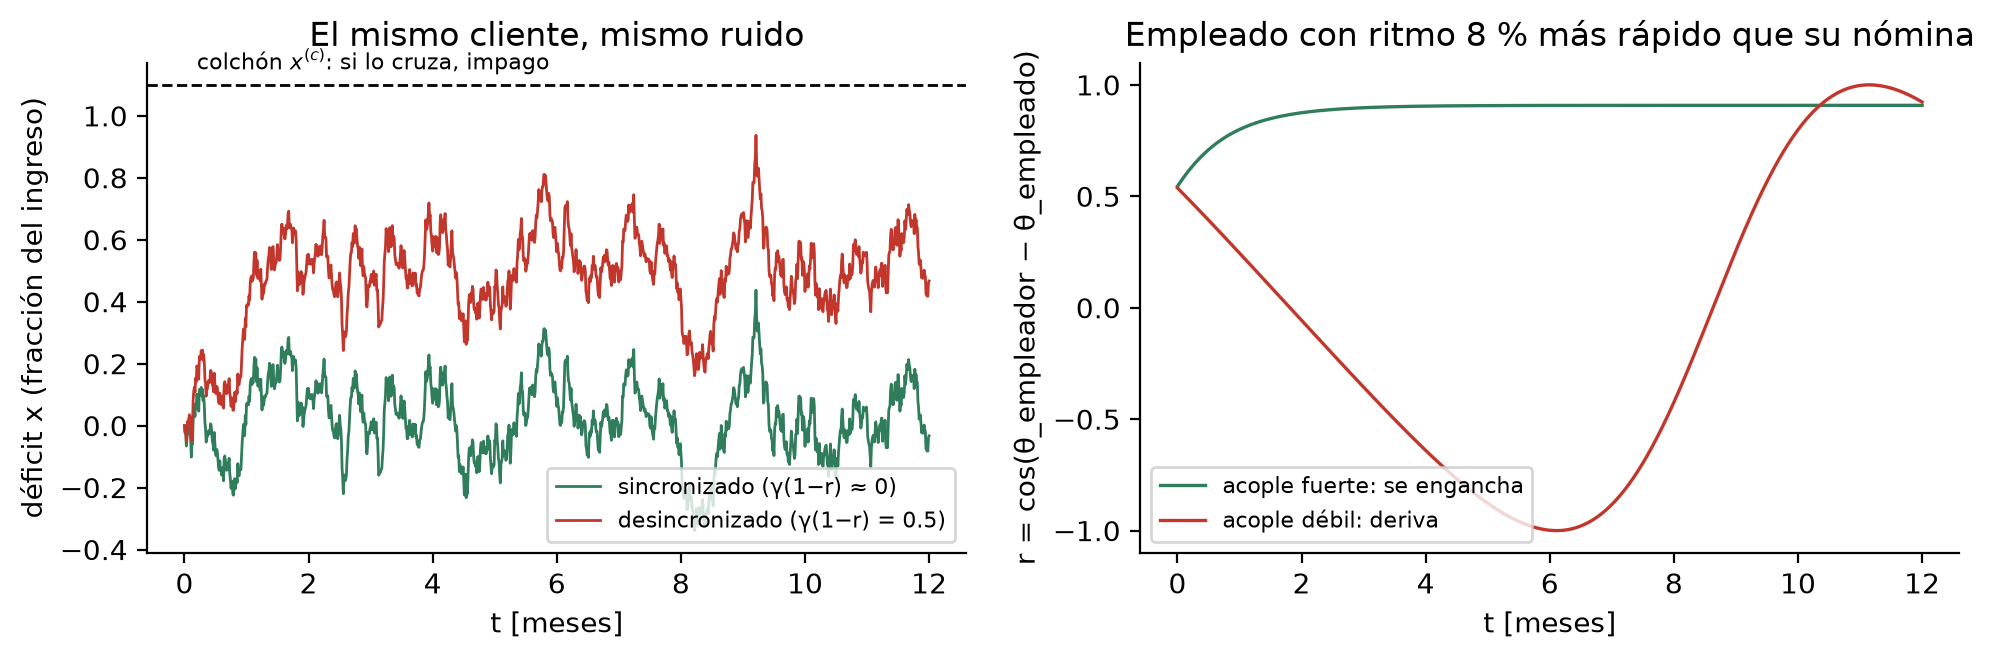
\includegraphics[width=\textwidth]{concepto_deficit_y_ritmo.png}
\caption{Izquierda: el mismo cliente con el mismo ruido; desincronizado, su déficit
vive más cerca del colchón y es más probable que lo cruce. Derecha: un empleado cuyo
ritmo natural es 8~\% más rápido que el de su nómina. Con acople fuerte se
``engancha'' (la coherencia $r$ se queda alta); con acople débil deriva y pasa por
momentos de desfase total ($r=-1$).}
\label{fig:concepto}
\end{figure}

\section{Del lenguaje físico al lenguaje financiero}
\begin{center}
\begin{tabular}{p{0.42\textwidth}p{0.48\textwidth}}
\toprule
\textbf{Física} & \textbf{Finanzas} \\
\midrule
Nodo de una red & Entidad, persona o empresa \\
Arista con peso $W_{ij}$ & Pago medio de $j$ hacia $i$ por ciclo \\
Variable de estado $x_i$ & Déficit de liquidez \\
Relajación ($-\alpha x$) & Capacidad de corregir el déficit \\
Acople lineal ($\beta W x$) & Contagio del déficit de quien me paga \\
Difusión (Laplaciano) & Redistribución de liquidez \\
Fase $\theta_i$ y frecuencia $\omega_i$ & Momento del ciclo de pagos y su ritmo \\
Parámetro de orden $r$ & Grado de sincronía de los pagos \\
Umbral $x_i^{(c)}$ & Colchón de liquidez \\
Avalancha / cascada & Contagio de impagos (riesgo sistémico) \\
Transición de fase & Paso de ``la red amortigua'' a ``la red amplifica'' \\
\bottomrule
\end{tabular}
\end{center}

% ---------------------------------------------------------------------------
\chapter{Impacto: para quién y para qué}

\section{Quién podría usarlo}
\begin{description}
\item[Supervisores y banco central.] Identificar qué entidades son sistémicamente
importantes (cuya caída arrastra más), simular choques (un retiro masivo de liquidez,
una caída tecnológica) y vigilar indicadores de alerta temprana como la sincronía
global de los pagos.
\item[Bancos.] Ver el \emph{riesgo oculto} de su cartera: clientes con buen score
cuyos ingresos dependen de pagadores frágiles o les llegan desfasados; y evaluar
escenarios como ``¿qué pasa con mis deudores si quiebra su empleador?''.
\item[Investigación.] Un puente concreto entre física estadística y finanzas, con
una hipótesis que se puede refutar.
\end{description}

\section{Qué es nuevo y qué no}
Es importante ser honestos sobre la novedad:
\begin{itemize}
\item \textbf{No es nuevo} usar la red para medir riesgo crediticio. Hay trabajos que
usan la red de pagos entre empresas para mejorar la calificación (Letizia y Lillo,
2019), redes de transacciones de pymes (Tobback et al., 2017) y contagio de firmas a
sus trabajadores (Banco Central de Brasil). Casi siempre usan la red de forma
\textbf{estática}: cuántos pagadores tiene un cliente, qué tan central es, si sus
vecinos han caído.
\item \textbf{Lo que parece nuevo} es usar la \textbf{dinámica}: tratar a cada
cliente como un oscilador cuyo ciclo de pagos se sincroniza (o no) con el de quienes
le pagan, medir esa sincronía desde las transacciones y probar si predice impagos más
allá de lo estático. La búsqueda bibliográfica hecha fue corta: antes de afirmarlo en
un documento formal debe hacerse una revisión sistemática.
\end{itemize}

\section{Qué no promete}
\begin{limite}
Los parámetros del modelo son \textbf{ilustrativos}: no están calibrados con datos
reales de ningún banco ni de Bre-B. El proyecto demuestra que el \emph{mecanismo} es
coherente, que se puede medir desde datos de transacciones y que el método de
evaluación separa la señal real de los artefactos. No demuestra que el mecanismo
exista en una cartera real: para eso hacen falta datos reales anonimizados de un
banco (en Colombia, bajo la Ley 1581 de 2012 de protección de datos).
\end{limite}

% ---------------------------------------------------------------------------
\chapter{Cómo funciona, en seis pasos}

\begin{figure}[h]
\centering
\begin{tikzpicture}[
  paso/.style={draw=azul,fill=azul!6,rounded corners=3pt,align=center,
    minimum width=3.6cm,minimum height=1.25cm,font=\sffamily\small},
  flecha/.style={-{Stealth[length=3mm]},thick,gris}]
\node[paso] (a) {1. Construir\\la red};
\node[paso,right=0.9cm of a] (b) {2. Diagnosticar:\\¿amortigua o amplifica?};
\node[paso,right=0.9cm of b] (c) {3. Ritmo de pagos:\\¿se sincronizan?};
\node[paso,below=1.1cm of c] (d) {4. Choque y\\cascada de impagos};
\node[paso,left=0.9cm of d] (e) {5. Miles de escenarios\\+ aprendizaje automático};
\node[paso,left=0.9cm of e,draw=rojo,fill=rojo!6] (f) {6. Cartera de un banco:\\riesgo crediticio};
\draw[flecha] (a)--(b); \draw[flecha] (b)--(c); \draw[flecha] (c)--(d);
\draw[flecha] (d)--(e); \draw[flecha] (e)--(f);
\end{tikzpicture}
\caption{Las seis tareas, en el orden en que se construyen. Cada una agrega un
ingrediente al mismo modelo; la última lo aplica al crédito.}
\label{fig:seis}
\end{figure}

\begin{enumerate}
\item \textbf{Construir la red.} Se genera una red de pagos sintética con una forma
realista: por ejemplo, \emph{núcleo-periferia}, con unas pocas entidades grandes muy
conectadas y muchas pequeñas que dependen de ellas.
\item \textbf{Diagnosticar.} Con matemática de matrices (valores propios) se calcula
un solo número, el \term{índice de amplificación} $R$. Si $R<1$ la red apaga los
choques; si $R>1$ los amplifica. También se calcula cuánto tarda en recuperarse.
\item \textbf{Ritmo de pagos.} Se simula cómo se sincronizan los ciclos de pago y
cuánto déficit genera la desincronización.
\item \textbf{Choque y cascada.} Se golpea una entidad (le quitamos liquidez o la
``apagamos'') y se observa quién cae después y cuánta plata queda sin pagar.
\item \textbf{Aprender.} Se corren 20\,000 escenarios distintos y con ellos se
entrenan modelos de aprendizaje automático que predicen el colapso en milisegundos,
en lugar de los segundos que tarda simular.
\item \textbf{Aplicar al crédito.} Se construye la cartera de un banco (personas y
empresas unidas por nómina, proveedores y transferencias), se simula, se genera el
registro de transacciones que vería el banco y se compara un score clásico con uno
que además mira la red y su sincronía.
\end{enumerate}

Todo esto vive en un programa en Python con una aplicación web (Streamlit) en la que
cada paso tiene su página: \emph{Construir red}, \emph{Diagnóstico}, \emph{Ritmo de
pagos}, \emph{Simulador de choques}, \emph{Explorar escenarios}, \emph{Mapa de
riesgo}, \emph{Cartera multicapa} y \emph{Riesgo crediticio híbrido}.

\part{La base desde cero}
% ===================================================================== PARTE II
\chapter{Matemática mínima}
Este capítulo reúne las cinco herramientas que usa todo el proyecto. Si ya las
conoce, puede saltarlo.

\section{Vectores y matrices}
Un \term{vector} es una lista de números: $x = (x_1, x_2, \dots, x_N)$, uno por
entidad. Una \term{matriz} es una tabla: $W_{ij}$ es el número en la fila $i$ y la
columna $j$. Multiplicar una matriz por un vector, $(Wx)_i = \sum_j W_{ij}x_j$,
significa: para cada $i$, sumar lo que aporta cada $j$ ponderado por $W_{ij}$. En la
red de pagos, si $x_j$ es el déficit de $j$ y $W_{ij}$ lo que $j$ le paga a $i$, entonces
$(Wx)_i$ mide cuánto déficit le ``llega'' a $i$ desde quienes le pagan.

\section{Ecuaciones diferenciales}
Una \term{ecuación diferencial} dice cómo \emph{cambia} una cantidad. La más simple:
\[
\frac{dx}{dt} = -\alpha x \quad\Longrightarrow\quad x(t) = x(0)\,e^{-\alpha t}.
\]
Si hoy me falta $x(0)$, cada día corrijo una fracción $\alpha$ de lo que me falta y el
déficit decae exponencialmente. El tiempo típico de recuperación es $1/\alpha$.

\section{Integrar en el computador: Euler y RK4}
Casi nunca hay fórmula cerrada; se avanza en pasos pequeños $\Delta t$. El método de
\term{Euler} usa $x(t+\Delta t)\approx x(t) + \Delta t\, f(x(t))$. El proyecto usa
\term{Runge–Kutta de orden 4} (RK4): evalúa la pendiente cuatro veces dentro del paso
y las promedia; el error baja como $\Delta t^4$, así que con $\Delta t=0.01$ es
despreciable.

\begin{codigo}[label=src/finnet/integrate.py]
def rk4_step(dyn: Dynamics, x, theta, source, dt):
    k1x, k1t = dyn.rhs(x, theta, source)
    k2x, k2t = dyn.rhs(x + 0.5 * dt * k1x, theta + 0.5 * dt * k1t, source)
    k3x, k3t = dyn.rhs(x + 0.5 * dt * k2x, theta + 0.5 * dt * k2t, source)
    k4x, k4t = dyn.rhs(x + dt * k3x, theta + dt * k3t, source)
    x_new = x + (dt / 6.0) * (k1x + 2 * k2x + 2 * k3x + k4x)
    th_new = theta + (dt / 6.0) * (k1t + 2 * k2t + 2 * k3t + k4t)
    return x_new, th_new
\end{codigo}

\section{Valores propios}
Para un sistema lineal $\dot x = Mx$, la solución es una mezcla de ``modos''
$e^{\lambda t}v$, donde $Mv=\lambda v$: $\lambda$ es un \term{valor propio} y $v$ su
\term{vector propio}. Si todos los $\lambda$ tienen parte real negativa, todo decae
(estable); si alguno es positivo, algo crece sin control (inestable). Así, \emph{un
solo número}, el mayor valor propio, decide si la red amortigua o amplifica.

\section{Fases y números complejos}
Una fase $\theta$ es un ángulo: la posición de la aguja de un reloj. Se representa con
el número complejo $e^{i\theta}=\cos\theta + i\sin\theta$, un punto en el círculo
unitario. El promedio de muchos de esos puntos, $\frac1N\sum_j e^{i\theta_j}$, tiene
longitud $r\in[0,1]$: $r=1$ si todas las agujas apuntan igual (sincronía total),
$r\approx0$ si apuntan a cualquier lado.

% ---------------------------------------------------------------------------
\chapter{Tarea 1 · La red y el déficit}

\section{La matriz de pagos $W$}
Toda la información de la red está en la matriz $W$ de tamaño $N\times N$.
\begin{nota}[Convención única del proyecto]
$W_{ij}$ es el pago medio \textbf{de $j$ hacia $i$} por ciclo. Las filas suman lo que
recibe cada entidad, $k_i = \sum_j W_{ij}$ (su \emph{ingreso}); las columnas suman lo
que paga, $\mathrm{out}_j=\sum_i W_{ij}$. Los montos se normalizan para que el pago
medio sea 1: la unidad de dinero es ``un pago medio por ciclo''.
\end{nota}

\begin{figure}[h]
\centering
\begin{tikzpicture}[n/.style={circle,draw=azul,fill=azul!10,minimum size=8mm,font=\sffamily},
  e/.style={-{Stealth[length=2.5mm]},thick}]
\node[n] (1) at (0,0) {1};
\node[n] (2) at (2.4,0.9) {2};
\node[n] (3) at (2.4,-0.9) {3};
\draw[e] (1) -- node[above,font=\small]{3} (2);
\draw[e] (2) -- node[right,font=\small]{1} (3);
\draw[e] (3) -- node[below,font=\small]{2} (1);
\node at (7,0) {$W=\begin{pmatrix}0&0&2\\3&0&0\\0&1&0\end{pmatrix}
\quad\begin{array}{l}\text{fila } i\text{: lo que recibe } i\\
\text{columna } j\text{: lo que paga } j\end{array}$};
\end{tikzpicture}
\caption{Una red de tres entidades. La entidad 1 le paga 3 a la 2, así que $W_{21}=3$.}
\end{figure}

\section{Formas de red}
\archivo{src/finnet/networks.py} genera tres familias clásicas:
\begin{itemize}
\item \term{Erdős–Rényi}: cada par se conecta al azar con la misma probabilidad. Es la
referencia ``sin estructura''.
\item \term{Barabási–Albert}: los nodos nuevos prefieren conectarse con los que ya
tienen muchas conexiones; aparecen ``hubs'' (como los grandes bancos).
\item \term{Núcleo-periferia}: un núcleo pequeño y denso (bancos grandes) y una
periferia que se conecta sobre todo con el núcleo. Es la forma observada en sistemas
de pagos reales.
\end{itemize}
Los montos son $W_{ij}=\sqrt{s_is_j}\,\varepsilon_{ij}$, con tamaños $s$ y ruido
$\varepsilon$ lognormales (pocos montos muy grandes, muchos pequeños):
\begin{codigo}[label=src/finnet/networks.py · generate]
sizes = rng.lognormal(0.0, cfg.amount_sigma, cfg.n)
noise = rng.lognormal(0.0, cfg.amount_sigma, (cfg.n, cfg.n))
W = np.where(A, np.sqrt(np.outer(sizes, sizes)) * noise, 0.0)
return normalize_weights(W)
\end{codigo}

\section{La ecuación del déficit}
La primera versión del modelo es lineal:
\[
\boxed{\;\frac{dx_i}{dt} = -\alpha\,x_i + \beta\sum_j W_{ij}\,x_j\;}
\]
\begin{itemize}
\item $-\alpha x_i$: \textbf{autocorrección}. Cada entidad corrige una fracción
$\alpha$ de su déficit por ciclo.
\item $\beta\sum_j W_{ij}x_j$: \textbf{contagio}. Si quien me paga está en déficit, me
paga menos o más tarde, y eso me crea déficit, en proporción a cuánto me paga
($W_{ij}$).
\end{itemize}

\section{El índice de amplificación $R$}
En forma matricial, $\dot x = (-\alpha I + \beta W)x$. Como $W$ no tiene números
negativos, el teorema de \term{Perron–Frobenius} garantiza que su valor propio más
grande es real y positivo: el \term{radio espectral} $\rho(W)$. El sistema es estable
si y solo si $-\alpha + \beta\rho(W) < 0$, es decir
\[
\boxed{\;R = \frac{\beta\,\rho(W)}{\alpha} < 1.\;}
\]
\begin{idea}
$R$ compara dos fuerzas: cuánto se contagia el déficit por la red ($\beta\rho$) contra
cuánto se corrige solo ($\alpha$). Es el análogo del ``número de reproducción'' de una
epidemia: con $R<1$ cada problema genera menos de un problema nuevo y se apaga.
\end{idea}

\begin{codigo}[label=src/finnet/spectral.py]
def perron_root(W: np.ndarray) -> float:
    """Valor propio dominante ρ(W) (real y no negativo para W >= 0)."""
    ev = np.linalg.eigvals(np.asarray(W, dtype=float))
    return float(np.max(ev.real)) if ev.size else 0.0

def amplification_index(W: np.ndarray, params: Params) -> float:
    """Índice de amplificación ``R = β ρ(W) / α``."""
    num = params.beta * perron_root(W)
    ...
    return num / params.alpha
\end{codigo}

Además, los vectores propios dominantes ordenan a las entidades: el vector
\emph{izquierdo} mide cuánto déficit \emph{propaga} cada una (importancia) y el
\emph{derecho} cuánto \emph{acumula} (vulnerabilidad).

\section{Parámetros y el modelo como objeto}
\archivo{src/finnet/model.py} define \texttt{Params}, un contenedor inmutable de los
parámetros: $\alpha,\beta$ (tarea 1), $D_0$ (tarea 2), $K,\gamma,\omega$ (tarea 3),
umbrales y pérdida $\lambda$ (tarea 4). Todos los términos nuevos valen cero por
defecto: \textbf{con los términos apagados, el modelo vuelve exactamente al de la
tarea anterior}. Esta regla de diseño es la que permite construir en capas y probar
cada capa por separado.

% ---------------------------------------------------------------------------
\chapter{Tarea 2 · Difusión y estabilidad}

\section{El Laplaciano: mover sin crear ni destruir}
La tarea 2 agrega la \term{redistribución}: la presión de liquidez se traslada por la
red (por ejemplo, alguien presta a quien le falta), pero el total no cambia. Eso lo
hace el \term{Laplaciano de flujo}
\[
L = D_\text{out} - W,\qquad \frac{dx}{dt} = -D_0\,L\,x,
\]
con $D_\text{out}$ la matriz diagonal de pagos salientes. Las columnas de $L$ suman
cero, por eso $\sum_i x_i$ se conserva: la difusión mueve déficit, no lo crea.

\section{El modelo con las dos piezas}
\[
\dot x = M x,\qquad M = -\alpha I - D_0 L + \beta W.
\]
\begin{itemize}
\item \term{Estabilidad} $\sigma = \max\mathrm{Re}\,\lambda(M)$: si $\sigma<0$ la red
se recupera de cualquier choque.
\item \term{Tiempo de recuperación} $\tau_\text{rec} = -1/\sigma$ (en ciclos).
\item \term{Conectividad algebraica} $\lambda_2$: el segundo valor propio del
Laplaciano simétrico. Mide qué tan bien conectada está la red; en redes simétricas
la tasa de recuperación es exactamente $\alpha + D_0\lambda_2$.
\end{itemize}

\section{Comunidades}
El vector propio asociado a $\lambda_2$ (vector de \term{Fiedler}) parte la red en dos
grupos poco conectados entre sí; repitiendo la partición se obtienen
\term{comunidades}. Se usa la versión \emph{normalizada} del Laplaciano (corte
normalizado de Shi y Malik, 2000), que da grupos balanceados en lugar de separar
unos pocos nodos periféricos.

\begin{codigo}[label=src/finnet/spectral.py]
def stability(W: np.ndarray, params: Params) -> float:
    """``σ = max Re λ(M)``; el sistema lineal es estable si σ < 0."""
    return float(spectrum(linear_operator(W, params))[0].real)

def recovery_time(W: np.ndarray, params: Params) -> float:
    """``τ_rec = -1/σ`` en ciclos; ``inf`` si σ >= 0 (no se recupera)."""
    sigma = stability(W, params)
    return -1.0 / sigma if sigma < 0 else float("inf")
\end{codigo}

% ---------------------------------------------------------------------------
\chapter{Tarea 3 · Sincronización: el modelo de Kuramoto}

\section{Osciladores}
Cada entidad tiene un ciclo de pagos, representado por una fase $\theta_i(t)$ que
avanza a su ritmo natural $\omega_i$ (una vuelta completa, $2\pi$, por ciclo). Si
dependo de los fondos de otros, ajusto mi ritmo al de ellos:
\[
\boxed{\;\frac{d\theta_i}{dt} = \omega_i + \frac{K}{\langle k\rangle}\sum_j W_{ij}\,
\sin(\theta_j-\theta_i)\;}
\]
El término $\sin(\theta_j-\theta_i)$ acelera a $i$ si $j$ va adelante y lo frena si va
atrás. $K$ es la fuerza del acople.

\section{Parámetro de orden y coherencia local}
\[
r = \Big|\frac1N\sum_j e^{i\theta_j}\Big|,\qquad
r_i = \frac{1}{k_i}\sum_j W_{ij}\cos(\theta_j-\theta_i).
\]
$r$ mide la sincronía global; $r_i$ mide si a la entidad $i$ el dinero le llega
\emph{en fase} ($r_i\approx1$) o desfasado ($r_i\le0$) respecto a su propio ciclo.

El resultado clásico de Kuramoto: con frecuencias repartidas según una distribución
de Lorentz de ancho $\Delta$, en la red completa hay sincronía parcial a partir de
$K_c=2\Delta$, con $r=\sqrt{1-2\Delta/K}$. El proyecto lo reproduce numéricamente (ver
capítulo de validación).

\section{La desincronización cuesta}
El puente entre el ritmo y el déficit es un término nuevo en la ecuación de $x$:
\[
\gamma\,k_i\,(1-r_i) = \gamma\sum_j W_{ij}\big(1-\cos(\theta_j-\theta_i)\big).
\]
Es el ingreso que llega desfasado, multiplicado por $\gamma$. Si todo llega en fase,
el término es cero; si llega en contrafase, cuesta $2\gamma k_i$.

\begin{nota}[Dos diferencias deliberadas con la propuesta]
(1) El acople se divide por el ingreso medio $\langle k\rangle$ y no por $N$: en redes
dispersas, $K/N$ hace desaparecer el acople cuando $N$ crece (forma de Rodrigues et
al., 2016). En la red completa ambas coinciden. (2) El término de desincronización es
proporcional al ingreso desfasado, no un número fijo: así es dimensionalmente
consistente (dinero por ciclo).
\end{nota}

\section{El modelo completo}
\[
\frac{dx_i}{dt} = -\alpha x_i + \beta\sum_j W_{ij}x_j - D_0(Lx)_i + \gamma k_i(1-r_i)
+ \eta_i(t),
\]
\[
\frac{d\theta_i}{dt} = \omega_i + \frac{K}{\langle k\rangle}\sum_j W_{ij}
\sin(\theta_j-\theta_i).
\]
En el código, todo el lado derecho se evalúa con \emph{un solo} producto de matrices
$W\,[x,\cos\theta,\sin\theta]$, lo que lo hace rápido:
\begin{codigo}[label=src/finnet/model.py · Dynamics.rhs]
c, s = np.cos(theta), np.sin(theta)
prod = self.W @ np.column_stack((x, c, s))
Wx, zr, zi = prod[:, 0], prod[:, 1], prod[:, 2]
dx = -self.diag * x + self.offdiag * Wx + source
if self.p.gamma > 0:
    # k_i (1 - r_i) = k_i - Σ_j W_ij cos(θ_j - θ_i)
    dx = dx + self.p.gamma * (self.k - (c * zr + s * zi))
# Im(e^{-iθ} z) = cos θ · Im z - sin θ · Re z
dth = self.omega + self.kur * (c * zi - s * zr)
\end{codigo}

% ---------------------------------------------------------------------------
\chapter{Tarea 4 · Impagos y cascadas}

\section{El umbral}
Cada entidad tiene un \term{colchón} $x_i^{(c)}$: un múltiplo de sus pagos salientes,
con algo de dispersión aleatoria. Si $x_i > x_i^{(c)}$, la entidad cae en impago:
\begin{enumerate}
\item deja de pagar: su columna en $W$ se anula;
\item quienes recibían de ella pierden ese ingreso, lo que les suma déficit
(parámetro $\lambda$, la pérdida);
\item esos saltos pueden hacer caer a otros \emph{en el mismo instante}, así que se
repite hasta que no aparece ningún impago nuevo (cascada instantánea).
\end{enumerate}

\begin{codigo}[label=src/finnet/integrate.py · simulate (detección de impagos)]
def detect_defaults(t: float) -> bool:
    """Aplica impagos (y sus saltos) hasta agotar la cascada instantánea."""
    if thresholds is None:
        return False
    changed = False
    while True:
        new = ~defaulted & (x > thresholds)
        if not new.any():
            return changed
        apply_defaults(np.flatnonzero(new), t, None)
        changed = True
\end{codigo}

\section{Choques}
\begin{itemize}
\item \term{Retiro de liquidez}: un salto en el déficit de la entidad chocada.
\item \term{Caída operativa}: la entidad recibe pero no paga durante $T$ ciclos (una
falla tecnológica); si no cruza su umbral, se recupera.
\item \term{Quiebra} (agregado en la tarea 6): la entidad cae en impago en $t_0$.
\end{itemize}

\section{Modelos clásicos de comparación}
\archivo{src/finnet/cascades.py} implementa tres modelos de la literatura para
contrastar con la dinámica:
\begin{itemize}
\item \term{Eisenberg y Noe (2001)}: qué fracción de sus deudas puede pagar cada
entidad cuando todas pagan lo máximo posible a la vez (vector de liquidación).
\item \term{DebtRank} (Battiston et al., 2012): cuánto estrés propaga una entidad, sin
contar dos veces el mismo camino.
\item \term{Watts (2002)}: una entidad cae si cae una fracción suficiente de sus
pagadores.
\end{itemize}

\section{Indicadores de riesgo}
\archivo{src/finnet/metrics.py} resume cada corrida: fracción de entidades en impago,
liquidez no pagada acumulada, tiempo hasta el primer contagio, colapso global (cae al
menos el 30~\%) e \term{importancia sistémica} de cada entidad (fracción media de
\emph{otras} que caen cuando se la choca).

% ---------------------------------------------------------------------------
\chapter{Tarea 5 · Experimentos y aprendizaje automático}

\section{Por qué aprender}
Simular un escenario tarda del orden de 0.1~s. Responder ``¿qué tan riesgosa es cada
entidad?'' exige simular un choque a cada una. Un modelo de aprendizaje automático
entrenado con miles de simulaciones responde en milisegundos.

\section{El dataset}
\archivo{src/finnet/experiments.py} corre la dinámica completa a partir de
\archivo{configs/sweep.yaml}:
\begin{itemize}
\item 300 redes (de 30 a 150 entidades, las tres topologías);
\item 20\,000 escenarios muestreados con un \term{hipercubo latino} (cubre el espacio
de 13 parámetros de forma pareja) y con más densidad cerca de $R=1$, donde ocurre la
transición;
\item una tabla por entidad con su tamaño de cascada cuando el choque empieza en ella.
\end{itemize}
Cada fila tiene su propia semilla: el dataset es \textbf{reproducible bit a bit}, sin
importar en qué orden ni con cuántos procesos se genere. Se guarda en formato
\term{Parquet} con un esquema validado (columnas, tipos y rangos).

\section{Los modelos}
\begin{itemize}
\item \term{Regresión logística}: el modelo más simple de probabilidad; una suma
ponderada de variables pasada por una curva en forma de S.
\item \term{XGBoost}: muchos árboles de decisión pequeños que se corrigen unos a otros
(\emph{gradient boosting}). Suele ser el mejor en datos tabulares.
\item \term{GCN} (Kipf y Welling, 2017): una red neuronal que trabaja directamente
sobre el grafo; cada nodo combina su información con la de sus vecinos.
\item \term{PINN} (Raissi et al., 2019): una red neuronal ``informada por la física''
que recupera los parámetros $\alpha,\beta,\gamma,K$ a partir de trayectorias, obligando
a que respete las ecuaciones del modelo.
\end{itemize}

\section{Evaluar sin hacer trampa}
\begin{itemize}
\item \term{GroupKFold por red}: se divide en 5 partes de modo que una misma red
nunca esté a la vez en entrenamiento y en prueba. Si no, el modelo ``memoriza'' la red.
\item \term{ROC-AUC}: probabilidad de que el modelo ponga a un caso positivo
por encima de uno negativo (0.5 = azar, 1 = perfecto).
\item \term{PR-AUC}: útil cuando los positivos son pocos.
\item \term{Brier} y \term{calibración}: si el modelo dice ``30~\%'', ¿ocurre el 30~\%
de las veces?
\item \term{SHAP}: cuánto aporta cada variable a cada predicción.
\end{itemize}

% ---------------------------------------------------------------------------
\chapter{Tarea 6 · Riesgo crediticio en una red multicapa}

\section{De entidades a clientes}
Las tareas 1–5 estudian una red de entidades abstractas. La tarea 6 baja al nivel de
los \textbf{clientes de un banco}. Hay dos tipos de nodo y tres capas de relaciones:

\begin{center}
\begin{tabular}{llll}
\toprule
Capa & Dirección & Ciclo & Contagio \\
\midrule
N · nómina & firma $\to$ persona & quincenal o mensual & la firma cae, cae el sueldo \\
S · proveedores & firma $\to$ firma & facturas & el cliente no paga al proveedor \\
T · transferencias & persona $\to$ persona & irregular & débil y difuso \\
\bottomrule
\end{tabular}
\end{center}

\begin{figure}[h]
\centering
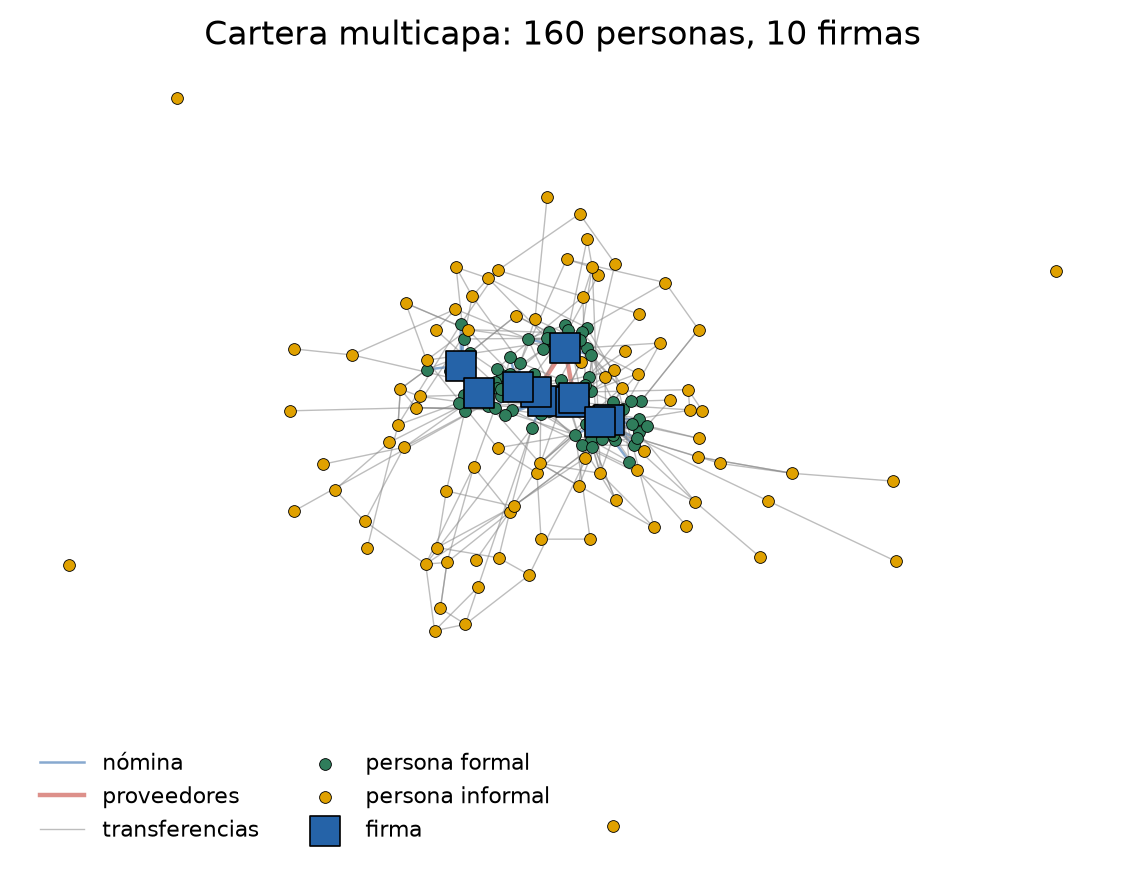
\includegraphics[width=0.85\textwidth]{tarea6_red_multicapa.png}
\caption{Una cartera pequeña. Cuadrados: firmas; círculos verdes: personas con
empleo formal; ámbar: informales. Azul: nómina; rojo: proveedores; gris:
transferencias.}
\end{figure}

\section{El mundo sintético: \texttt{finnet.world}}
No hay datos públicos con la red de pagos de los clientes de un banco, así que se
\emph{genera} una cartera realista con un mecanismo conocido. Eso permite comprobar
que el método recupera lo que debe.

\begin{itemize}
\item \archivo{world/entities.py}: 2000 personas y 100 firmas.
  \begin{itemize}
  \item 55~\% de las personas son informales (sin empleador en la red), del orden de
  la informalidad en Colombia según el DANE.
  \item El tamaño de las firmas sigue una ley de Pareto: pocas firmas grandes emplean
  a mucha gente.
  \item Variables clásicas: ingreso (en salarios mínimos por mes), endeudamiento,
  edad, antigüedad en el banco, número de productos, moras en 12 meses, empleo formal.
  \item Ritmos: las firmas pagan nómina mensual o quincenal; los formales heredan el
  ritmo de su empleador con poca dispersión; los informales tienen ritmos dispersos.
  \end{itemize}
\item \archivo{world/layers.py}: construye las tres capas. La nómina conecta a cada
formal con su único empleador; los proveedores siguen una matriz insumo-producto
entre sectores; las transferencias prefieren compañeros de trabajo y personas de la
misma comunidad.
\item \archivo{world/transactions.py}: el registro de pagos (más abajo).
\end{itemize}

\subsection{La verdad del terreno}
Cada cliente tiene una PD anual verdadera:
\[
\mathrm{logit}(\mathrm{PD}_i) = b + \sum_k c_k\,z_k(i) + \sigma_u\,u_i,
\]
donde $z_k$ son las variables clásicas estandarizadas y $u_i$ un componente
\emph{latente} que ningún dato muestra del todo (la mora observada lo revela solo en
parte, como el historial real). $b$ se ajusta para que la PD media sea 5~\% en personas
y 3~\% en firmas. Estas columnas se llaman \texttt{truth\_*} y una regla del código
impide que lleguen a un modelo:

\begin{codigo}[label=src/finnet/schema.py]
def assert_no_truth(columns) -> None:
    """Falla si alguna columna es verdad del terreno (fuga de información)."""
    leaked = [c for c in columns if str(c).startswith(TRUTH_PREFIX)]
    if leaked:
        raise ValueError(
            f"Columnas de verdad del terreno no pueden entrar a un modelo: {leaked}"
        )
\end{codigo}

\section{El motor multicapa}
El motor de las tareas 1–4 se generaliza sin romperlo. Con varias capas $\ell$ y el
tiempo medido en \textbf{meses}:
\[
\dot x_i = -\alpha x_i + \sum_\ell \beta_\ell\sum_j\frac{W^\ell_{ij}}{s_i}x_j
+ \gamma\,\frac{k_i}{s_i}(1-r_i) + \sigma\,\xi_i(t),
\]
\[
\dot\theta_i = \omega_i + \sum_\ell K_\ell \sum_j \frac{W^\ell_{ij}}{k_i}\sin(\theta_j-\theta_i).
\]
\begin{itemize}
\item $x_i$ ahora es \textbf{adimensional}: el déficit como fracción del ingreso total
$s_i$ (que incluye lo que llega de fuera de la red). Así una persona y una empresa son
comparables.
\item Cada capa tiene su propio contagio $\beta_\ell$ y su propio acople $K_\ell$.
\item El acople de fase se normaliza por fila: cada cliente ajusta su ritmo según la
participación de cada pagador en su ingreso.
\item $\sigma\xi_i(t)$ es ruido: pequeños choques de liquidez aleatorios (integrado con
el esquema de Euler–Maruyama).
\item El colchón depende de la PD verdadera,
$x_i^{(c)} = c\,(\mathrm{PD}_\text{ref}/\mathrm{PD}_i)^{\kappa}\,\varepsilon_i$: quien
es más riesgoso tiene menos margen.
\item Impagos \textbf{idiosincráticos}: cada cliente cae por sus propias razones en un
instante aleatorio con tasa $-\ln(1-\mathrm{PD}_i)/12$ por mes.
\end{itemize}

En el código, estas matrices se empaquetan en un objeto \texttt{Coupling}. Si no se
pasa, el motor es \emph{bit a bit} el de la versión 1 (lo verifica una prueba):
\begin{codigo}[label=src/finnet/model.py · Dynamics.\_rhs\_coupled]
cpl = self.coupling
dx = -self.p.alpha * x + cpl.stress @ x + source
if not self.need_phases:
    return dx, self.omega
c, s = np.cos(theta), np.sin(theta)
cs = np.column_stack((c, s))
if self.p.gamma > 0:
    zw = self.W @ cs
    # (k_i / s_i)(1 - r_i) = (k_i - Σ_j W_ij cos(θ_j - θ_i)) / s_i
    dx = dx + self.gamma_scale * (self.k - (c * zw[:, 0] + s * zw[:, 1]))
zc = cpl.phase @ cs
dth = self.omega + (c * zc[:, 1] - s * zc[:, 0])
\end{codigo}
Las matrices son \term{dispersas} (\texttt{scipy.sparse}): con 2100 clientes hay unas
5\,000 relaciones y no 4.4 millones de casillas, y una cartera completa se simula en
menos de un segundo.

\section{Lo que ve el banco: el registro de transacciones}
El banco no ve fases ni ritmos naturales. Ve \emph{pagos con fecha}. El simulador los
produce así: cada vez que la fase de un pagador cruza un múltiplo de $2\pi$, ejecuta
su ciclo de pagos y paga a cada receptor (más un pequeño ruido en el día y el monto) y
paga su cuota al banco. Quien cae en impago deja de pagar.

\section{Estimar desde las transacciones}
\archivo{src/finnet/credit/estimate.py} hace lo que haría un analista con los datos
reales:
\begin{enumerate}
\item $\hat W$: cuánto le paga cada pagador a cada receptor por mes (mientras pagó).
\item \textbf{Fase por eventos} (Pikovsky, Rosenblum y Kurths, 2001): si $t_k$ son los
instantes de los ciclos de pago de un cliente,
\[
\hat\theta(t) = 2\pi\Big(k + \frac{t-t_k}{t_{k+1}-t_k}\Big),\qquad t_k\le t<t_{k+1}.
\]
\item $\hat r_i(t)$: la coherencia local con las fases estimadas de sus pagadores.
\end{enumerate}
\begin{codigo}[label=src/finnet/credit/estimate.py · event\_phase]
k = np.searchsorted(times, grid, side="right") - 1
inside = (k >= 0) & (k < times.size - 1)
ki = k[inside]
theta[inside] = TWO_PI * (
    ki + (grid[inside] - times[ki]) / (times[ki + 1] - times[ki])
)
\end{codigo}

\begin{figure}[h]
\centering
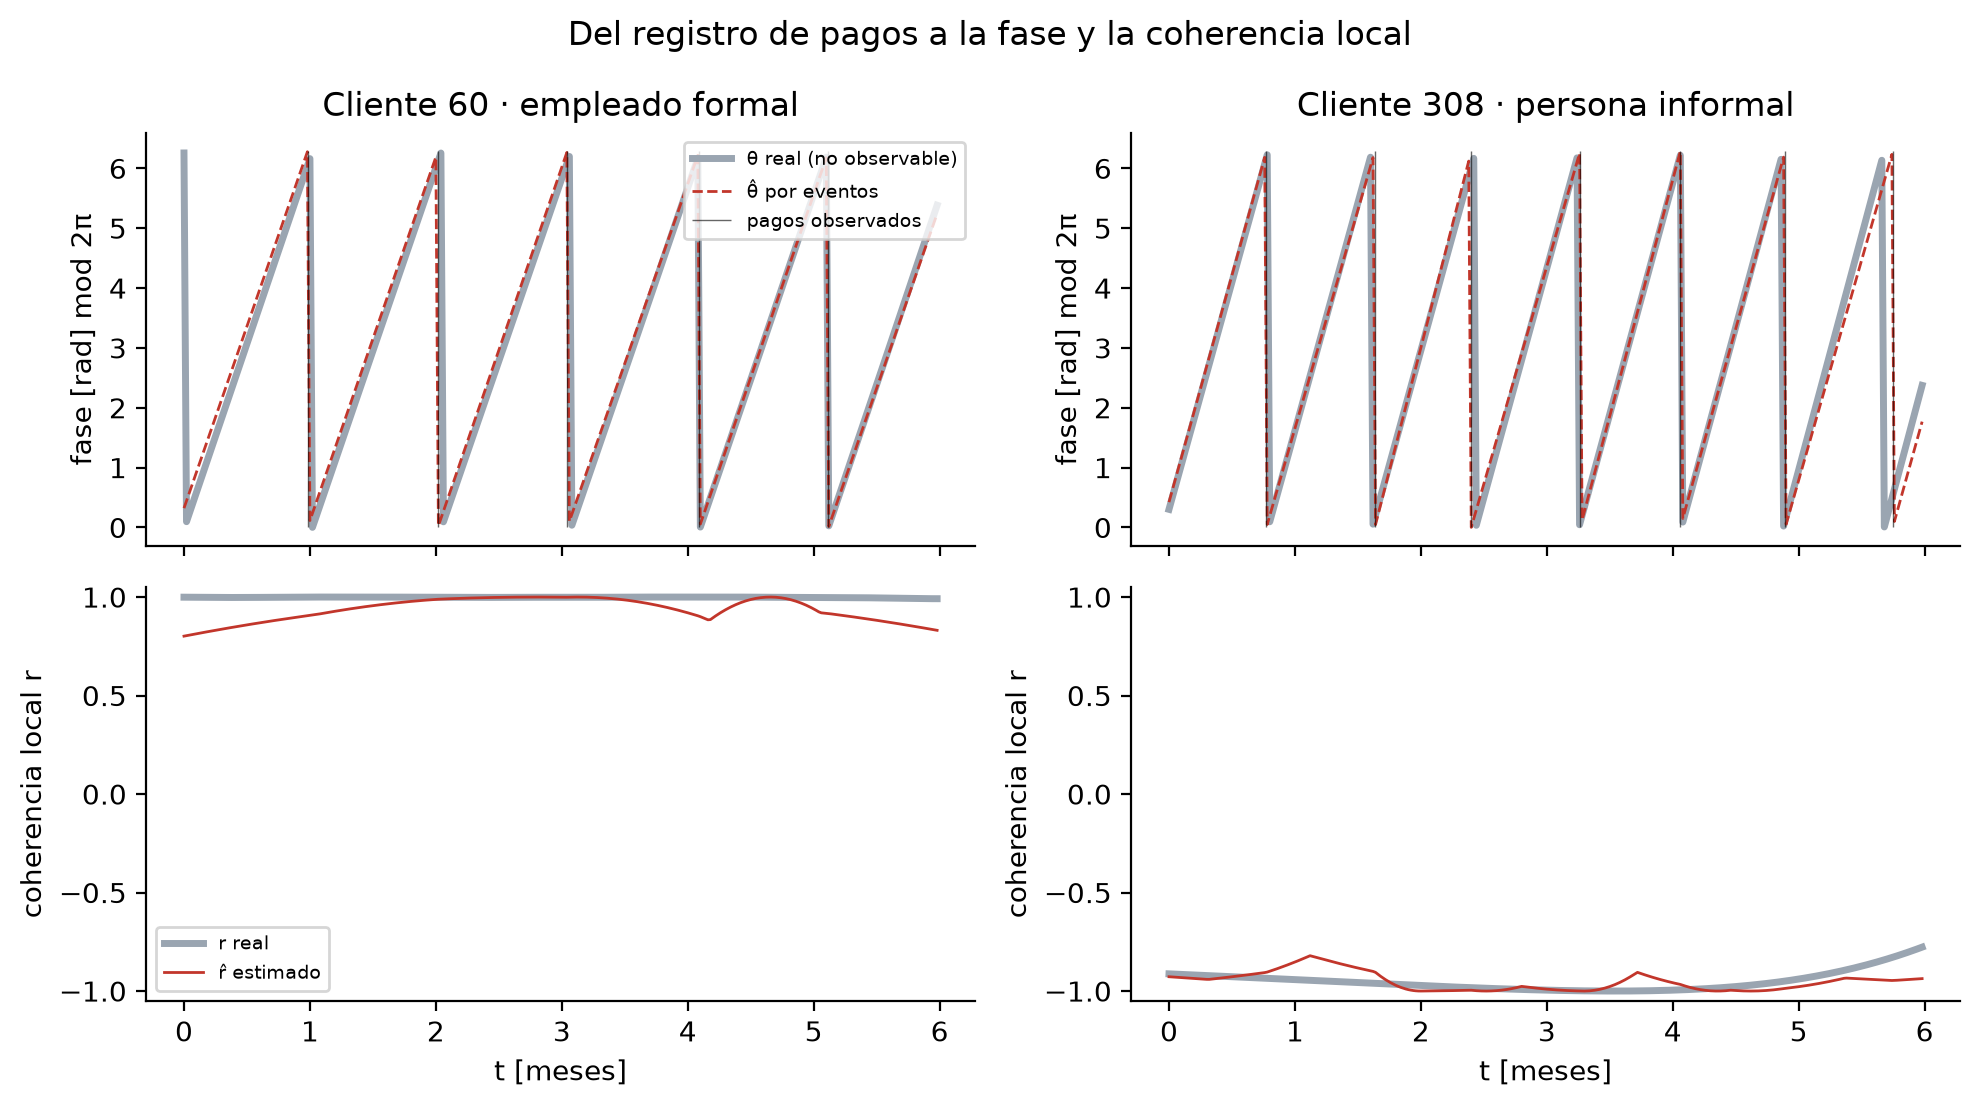
\includegraphics[width=\textwidth]{tarea6_fase_eventos.png}
\caption{Arriba: la fase real (gris, no observable) y la estimada solo con los pagos
(rojo), para un empleado formal y una persona informal. Abajo: su coherencia local
real y estimada. El formal está en fase con su empleador ($r\approx1$); la informal
recibe en contrafase ($r\approx-1$): el dinero le llega justo cuando no le sirve.}
\end{figure}

\section{Tres niveles de variables}
\archivo{src/finnet/credit/features.py} construye, para cada cliente y solo con los
primeros 6 meses de datos:
\begin{description}
\item[1 · Clásico.] Ingreso, endeudamiento, edad, antigüedad, productos, moras, empleo
formal, tamaño (firmas). Lo que usa cualquier score.
\item[2 · + Red estática.] Qué parte del ingreso llega por nómina, proveedores o
transferencias; número de pagadores; concentración del ingreso; PageRank; tamaño,
endeudamiento y moras del empleador; riesgo medio de los pagadores. Es lo que ya
explora la literatura.
\item[3 · + Red dinámica.] Coherencia local media $\hat r$, su variabilidad, tiempo
desincronizado ($\hat r<0.5$), desfase con los pagadores, desajuste de ritmo,
irregularidad de los ciclos propios y de los pagadores, e ingreso de pagadores que
dejaron de pagar. \textbf{Este es el aporte.}
\end{description}
La etiqueta es: ¿el cliente cae en impago en los 12 meses siguientes? Quien ya cayó
durante la observación se excluye.

\section{Evaluar con un control}
\archivo{src/finnet/credit/evaluate.py} y \archivo{experiment.py}:
\begin{itemize}
\item \textbf{Dos mundos}. En el mundo \emph{con red} los acoples están encendidos. En
el mundo \emph{nulo} ($\beta_\ell=\gamma=\lambda=0$) la red no crea déficit, pero los
clientes, las redes y \emph{todos los sorteos aleatorios} son idénticos (cuatro flujos
aleatorios independientes derivados de la misma semilla). Si en el mundo nulo las
variables de red ``mejoraran'' la predicción, habría una fuga de información.
\item \textbf{20 mundos por régimen}, \term{GroupKFold} por mundo (nunca se entrena y
evalúa con clientes del mismo mundo).
\item \textbf{Diferencias pareadas}: mismas filas, mismo modelo, misma partición; solo
cambian las variables. Se reporta la mejora media con su intervalo de confianza del
95~\%.
\end{itemize}
\begin{codigo}[label=src/finnet/credit/evaluate.py · paired\_deltas]
ref = cv[(cv["model"] == model) & (cv["level"] == base)].set_index("fold")
d = g.set_index("fold")[metric] - ref[metric]
k = len(d)
half = stats.t.ppf(0.975, k - 1) * d.std(ddof=1) / np.sqrt(k) if k > 1 else 0
\end{codigo}

% ---------------------------------------------------------------------------
\chapter{Cómo se une todo}

\section{Arquitectura en capas}
\begin{figure}[h]
\centering
\begin{tikzpicture}[
  caja/.style={draw=#1,fill=#1!7,rounded corners=3pt,align=left,
    minimum width=13cm,font=\sffamily\small,inner sep=6pt},
  flecha/.style={-{Stealth[length=3mm]},thick,gris}]
\node[caja=azul] (app) {\textbf{Interfaz} · \texttt{app/} (Streamlit): \texttt{Inicio.py} y nueve páginas.\\
Solo muestra; nunca calcula física.};
\node[caja=verde,below=0.6cm of app] (srv) {\textbf{Servicio} · \texttt{finnet/service.py} (tareas 1–5) y \texttt{finnet/credit/service.py} (tarea 6).\\
Recibe diccionarios de configuración; devuelve tablas y arreglos listos para mostrar.};
\node[caja=rojo,below=0.6cm of srv] (core) {\textbf{Núcleo} · \texttt{networks, model, integrate, spectral, cascades, metrics,}\\
\texttt{experiments, ml/} (tareas 1–5) · \texttt{world/, credit/} (tarea 6).\\
La física, la estimación y los modelos. Todo con pruebas.};
\node[caja=ambar,below=0.6cm of core] (cfg) {\textbf{Configuración y datos} · \texttt{configs/*.yaml}, \texttt{data/}, \texttt{models/}.\\
Ningún número del modelo está escrito en el código.};
\draw[flecha] (app)--(srv); \draw[flecha] (srv)--(core); \draw[flecha] (core)--(cfg);
\end{tikzpicture}
\caption{Cada capa solo habla con la de abajo. Una API web, por ejemplo, se montaría
sobre la capa de servicio sin tocar la física.}
\end{figure}

\section{El flujo de la tarea 6}
\begin{figure}[h]
\centering
\begin{tikzpicture}[
  p/.style={draw=azul,fill=azul!6,rounded corners=3pt,align=center,
    minimum width=2.9cm,minimum height=1.1cm,font=\sffamily\scriptsize},
  f/.style={-{Stealth[length=2.5mm]},thick,gris}]
\node[p] (w) {\texttt{world.yaml}\\generate\_world};
\node[p,right=0.5cm of w] (m) {motor multicapa\\run\_credit};
\node[p,right=0.5cm of m] (t) {registro de pagos\\emit\_transactions};
\node[p,right=0.5cm of t] (e) {estimación\\$\hat W$, $\hat\theta$, $\hat r$};
\node[p,below=0.8cm of e] (v) {variables\\3 niveles};
\node[p,left=0.5cm of v] (cv) {GroupKFold\\por mundo};
\node[p,left=0.5cm of cv] (d) {mejoras pareadas\\+ control nulo};
\node[p,left=0.5cm of d,draw=rojo,fill=rojo!6] (o) {resultados y\\modelos finales};
\draw[f] (w)--(m); \draw[f] (m)--(t); \draw[f] (t)--(e); \draw[f] (e)--(v);
\draw[f] (v)--(cv); \draw[f] (cv)--(d); \draw[f] (d)--(o);
\end{tikzpicture}
\caption{Un mundo entra por la izquierda; lo que sale a la derecha es lo que
muestra la página \emph{Riesgo crediticio híbrido}. Todo el flujo corre con un
comando: \texttt{uv run finnet credit configs/credit.yaml}.}
\end{figure}

\section{Reglas que mantienen todo coherente}
\begin{enumerate}
\item \textbf{Una sola convención}: $W_{ij}$ es lo que $j$ le paga a $i$, en todo el
código.
\item \textbf{Capas que se apagan}: con los términos nuevos en cero, el modelo es el
de la tarea anterior (y hay pruebas que lo verifican).
\item \textbf{Configuración externa}: todo parámetro vive en un archivo YAML de
\texttt{configs/}.
\item \textbf{Semillas explícitas}: misma configuración y semilla, mismo resultado.
\item \textbf{Esquemas validados}: las tablas que se guardan o entran a un modelo se
revisan (columnas, tipos, rangos) y la verdad del terreno está vetada.
\item \textbf{Pruebas}: 127 pruebas automáticas, muchas contra resultados analíticos.
\end{enumerate}

\section{Mapa de módulos}
\begin{longtable}{p{0.36\textwidth}p{0.58\textwidth}}
\toprule
\textbf{Archivo} & \textbf{Qué hace} \\
\midrule
\endhead
\archivo{networks.py} & Genera redes (Erdős–Rényi, Barabási–Albert, núcleo-periferia) \\
\archivo{model.py} & Parámetros, lado derecho de las ecuaciones, acoples multicapa \\
\archivo{integrate.py} & Integrador RK4, choques, impagos, ruido \\
\archivo{spectral.py} & $\rho(W)$, $R$, $\sigma$, $\tau_\text{rec}$, $\lambda_2$, comunidades \\
\archivo{cascades.py} & Eisenberg–Noe, DebtRank, Watts \\
\archivo{metrics.py} & $r$, $r_i$, fracción en impago, importancia sistémica \\
\archivo{experiments.py} & Barrido de 20\,000 escenarios y dataset (tarea 5) \\
\archivo{ml/train.py}, \archivo{gnn.py}, \archivo{predict.py}, \archivo{pinn.py}, \archivo{registry.py} & Modelos de la tarea 5, versionado y predicción \\
\archivo{service.py} & Fachada de las tareas 1–5 para la app \\
\archivo{schema.py} & Validación de tablas y veto de la verdad del terreno \\
\archivo{config.py} & Lectura de los YAML y rutas de datos y modelos \\
\archivo{cli.py} & Comandos \texttt{finnet sweep | train | world | credit} \\
\archivo{viz.py} & Figuras Plotly de la app \\
\archivo{world/} & Mundo multicapa: entidades, capas, transacciones \\
\archivo{credit/engine.py} & Acoples por capa, colchones, impagos idiosincráticos \\
\archivo{credit/estimate.py} & $\hat W$, fase por eventos, $\hat r_i$ \\
\archivo{credit/features.py} & Variables de los tres niveles \\
\archivo{credit/pipeline.py} & De un mundo a su tabla de clientes \\
\archivo{credit/evaluate.py} & Validación cruzada, métricas, mejoras pareadas \\
\archivo{credit/experiment.py} & El experimento completo y los modelos finales \\
\archivo{credit/service.py} & Fachada de la tarea 6 para la app \\
\bottomrule
\end{longtable}

\part{Resultados}
% ===================================================================== PARTE III
\chapter{Validación numérica}

Antes de creer un resultado hay que saber que el código calcula lo que dice. Las
pruebas automáticas (\archivo{tests/}) comparan el código con resultados conocidos de
antemano:

\begin{longtable}{p{0.45\textwidth}p{0.47\textwidth}}
\toprule
\textbf{Qué se verifica} & \textbf{Resultado} \\
\midrule
\endhead
RK4 contra la solución exacta $e^{Mt}x_0$ & error relativo $<10^{-6}$ \\
Conservación de $\sum_i x_i$ con difusión pura & variación $<10^{-10}$ \\
Tasa de recuperación $\alpha+D_0\lambda_2$ en redes simétricas & coincide al 1~\% \\
Kuramoto en red completa, Lorentz, $K=2$ & $r=0.7076$ simulado vs.\ $0.7071$ teórico \\
Eisenberg–Noe en un caso resuelto a mano & exacto \\
Dataset de la tarea 5 & idéntico bit a bit al regenerarlo \\
Motor multicapa con una capa vs.\ motor v1 & idénticos (error $<10^{-10}$) \\
Ruido: varianza estacionaria de Ornstein–Uhlenbeck $\sigma^2/2\alpha$ & coincide al 10~\% \\
Flujos estimados $\hat W$ vs.\ $W$ verdadero & error mediano $<5$~\% \\
Ritmos estimados desde pagos vs.\ verdaderos & error mediano $<5$~\% \\
Coherencia $\hat r_i$ estimada vs.\ $r_i$ del modelo & correlación $>0.8$ \\
Tasa de impago generada vs.\ objetivo & exacta por construcción (bisección) \\
Columnas \texttt{truth\_*} hacia un modelo & error inmediato \\
Cada página de la app & carga sin excepciones \\
\bottomrule
\end{longtable}

En total, 127 pruebas pasan (\texttt{uv run pytest}).

% ---------------------------------------------------------------------------
\chapter{Resultados de las tareas 1 a 5}

\section{Tarea 1: frontera de estabilidad $R=1$}
\begin{figure}[h]
\centering
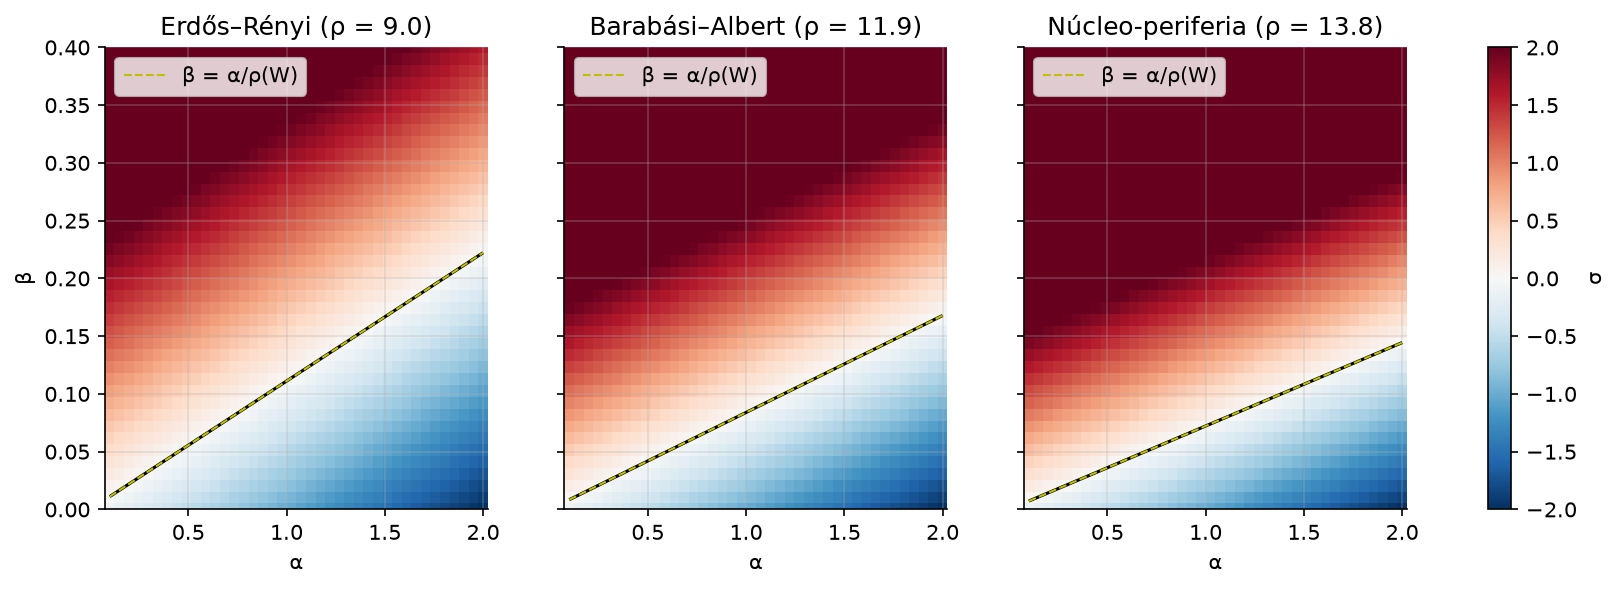
\includegraphics[width=\textwidth]{fase1_diagrama_alpha_beta.png}
\caption{Estabilidad en el plano $(\alpha,\beta)$ para las tres topologías. La línea
punteada es $\beta=\alpha/\rho(W)$, es decir $R=1$: por debajo la red amortigua (azul),
por encima amplifica (rojo). Las redes más concentradas (mayor $\rho$) se vuelven
inestables antes.}
\end{figure}
\begin{figure}[h]
\centering
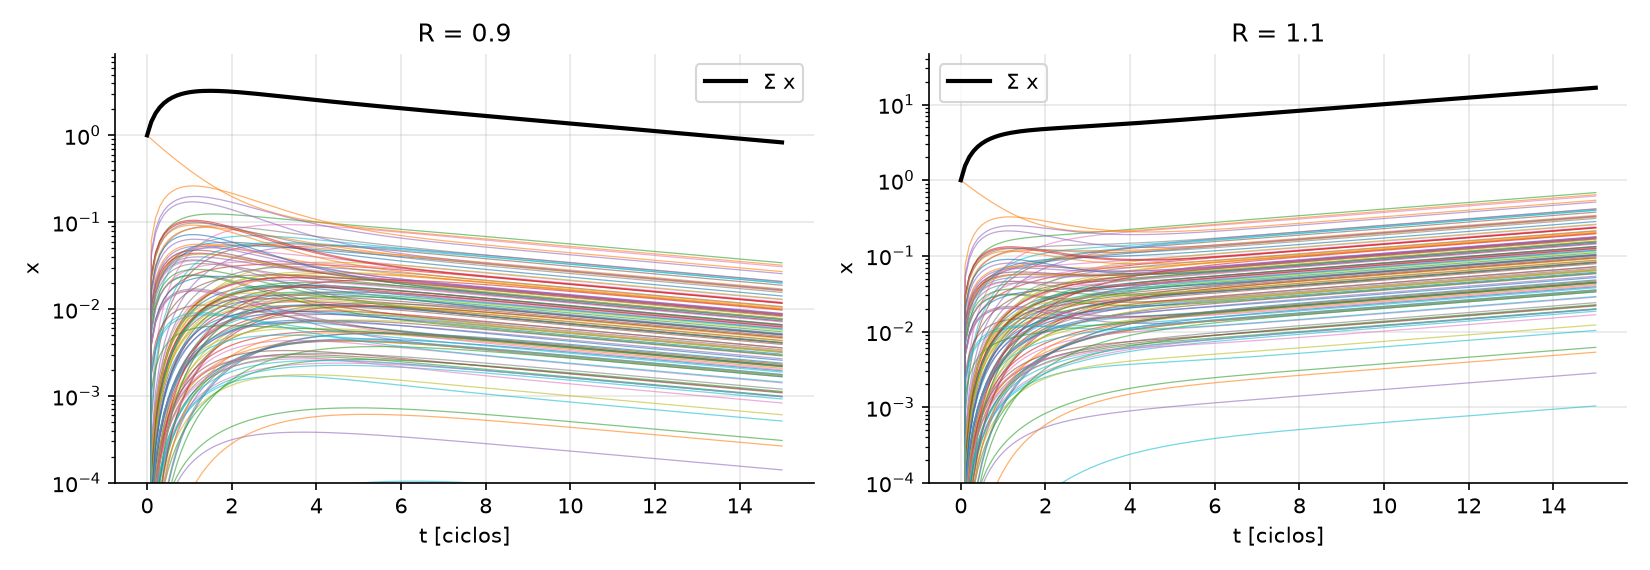
\includegraphics[width=0.9\textwidth]{fase1_trayectorias.png}
\caption{Déficit de cada entidad tras un choque con $R=0.9$ (se apaga) y $R=1.1$
(crece).}
\end{figure}

\section{Tarea 2: efecto estabilizador de la redistribución}
\begin{figure}[h]
\centering
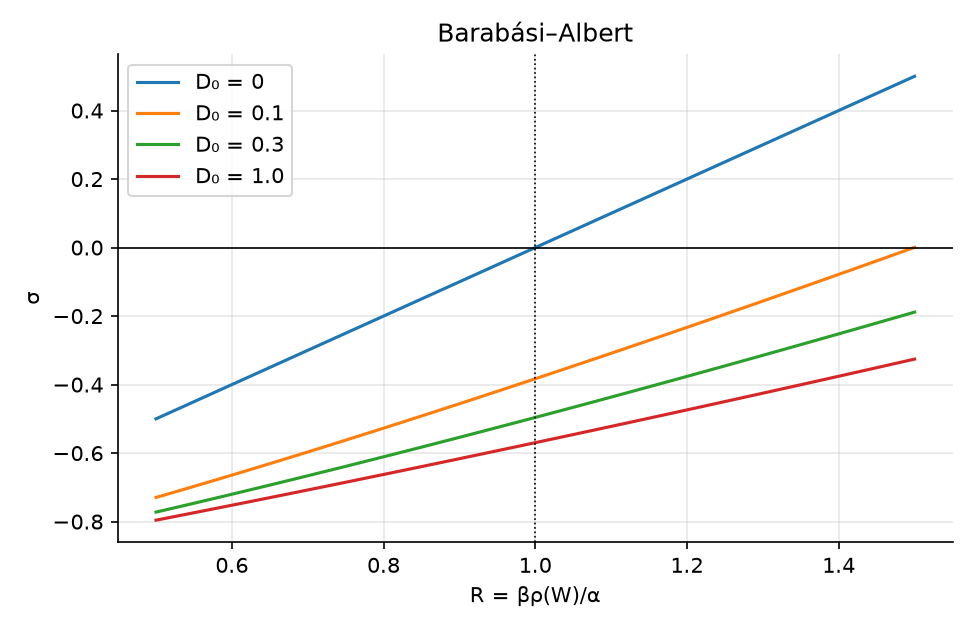
\includegraphics[width=0.48\textwidth]{fase2_D0_umbral.png}\hfill
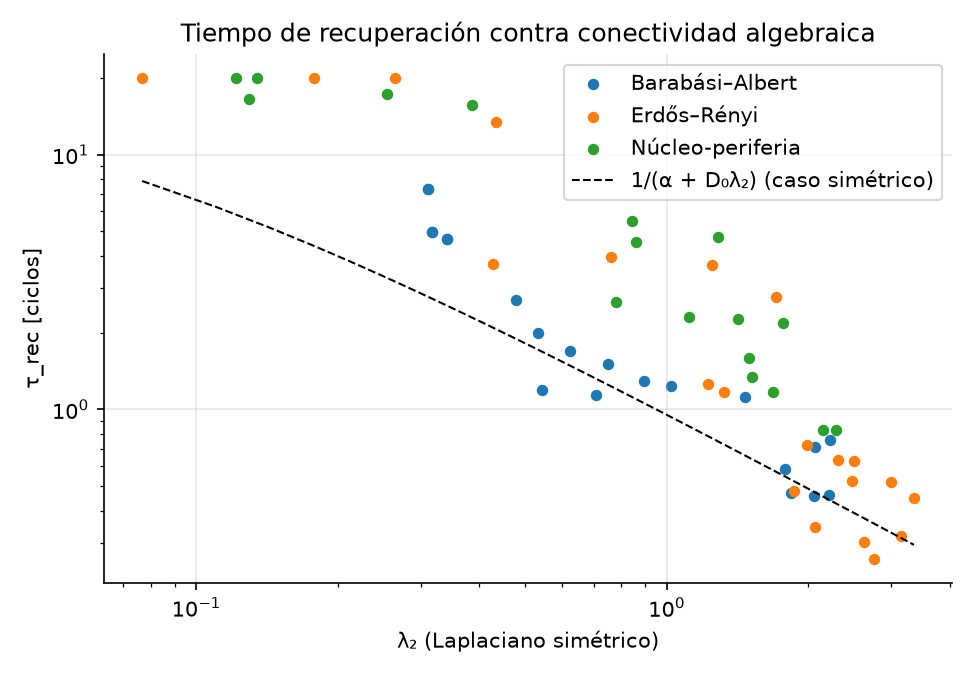
\includegraphics[width=0.48\textwidth]{fase2_tau_vs_lambda2.png}
\caption{Izquierda: con más redistribución $D_0$ la estabilidad $\sigma$ baja y la red
soporta valores de $R$ mayores que 1. Derecha: el tiempo de recuperación cae con la
conectividad algebraica $\lambda_2$; la línea es la predicción exacta del caso
simétrico.}
\end{figure}

\section{Tarea 3: transición de sincronización}
\begin{figure}[h]
\centering
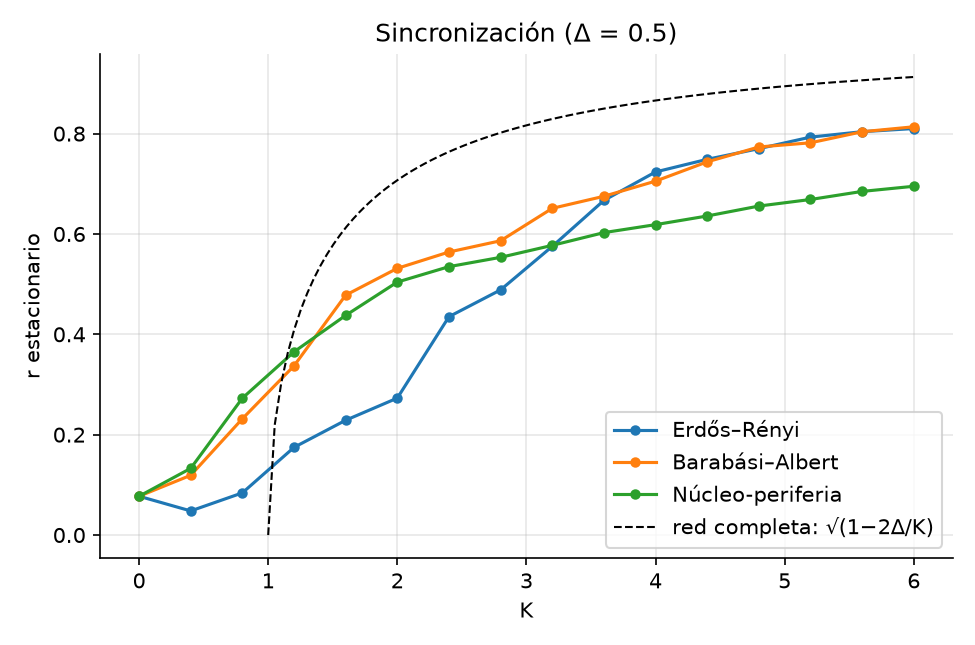
\includegraphics[width=0.6\textwidth]{fase3_r_vs_K.png}
\caption{Sincronía $r$ contra el acople $K$. La curva punteada es la solución
analítica de la red completa; las redes reales se sincronizan de forma más gradual.}
\end{figure}

\section{Tarea 4: cascadas de impago}
\begin{figure}[h]
\centering
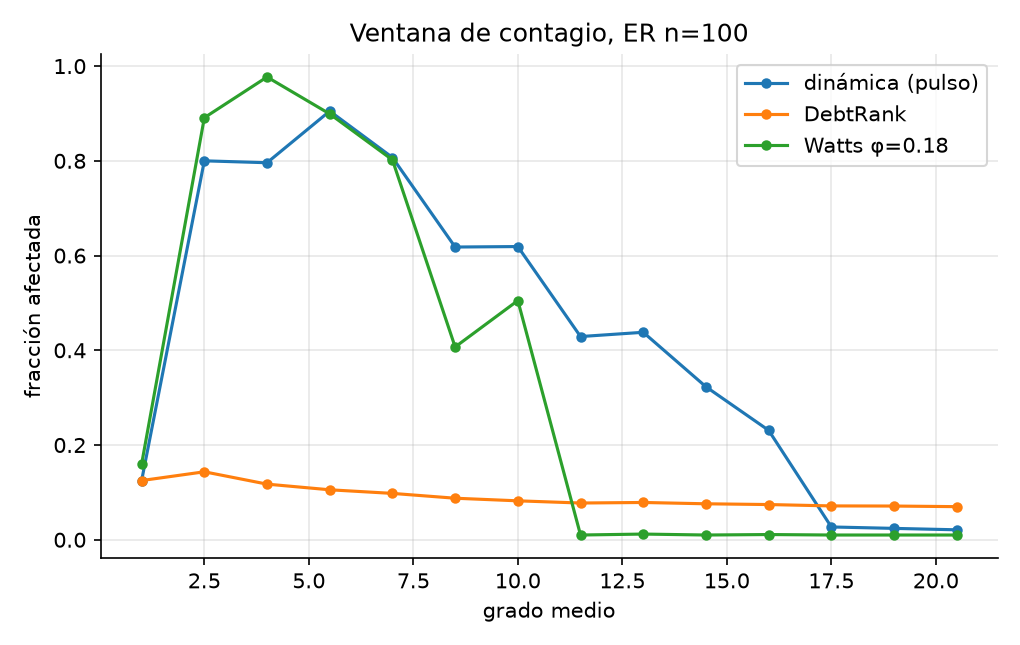
\includegraphics[width=0.55\textwidth]{fase4_ventana_contagio.png}
\caption{``Ventana de contagio'': fracción afectada contra el grado medio. Con pocas
conexiones el choque no se propaga; con muchas, cada entidad tiene suficientes
pagadores para absorber una pérdida; en medio, las cascadas son grandes. La dinámica
del proyecto, DebtRank y Watts muestran formas distintas.}
\end{figure}

\section{Tarea 5: desempeño predictivo}
\begin{center}
\begin{tabular}{llll}
\toprule
Modelo & Qué predice & Métricas (fuera de muestra) & Tiempo \\
\midrule
Regresión logística & colapso global & ROC-AUC 0.957 · PR-AUC 0.741 & 0.2 ms \\
XGBoost & colapso global & ROC-AUC \textbf{0.980} · PR-AUC \textbf{0.880} & 0.2 ms \\
XGBoost & cascada por entidad & $R^2$ 0.50 · Spearman intra-red 0.30 & 0.5 ms/red \\
GCN & cascada por entidad & $R^2$ \textbf{0.60} · Spearman intra-red 0.29 & 0.7 ms/red \\
\bottomrule
\end{tabular}
\end{center}
Una simulación cuesta $\sim$0.09~s por escenario: los modelos son unas $10^4$ veces más
rápidos. La PINN recupera $\gamma$ y $K$ con error menor al 1~\%, $\alpha$ al 7~\% y $\beta$
al 23~\% (el peor identificado, porque su efecto se confunde con el de $\alpha$).
\begin{limite}
Los modelos de entidades aciertan el \emph{nivel} de riesgo de una red, pero ordenan
solo moderadamente a las entidades dentro de ella (Spearman $\approx0.3$). Por eso la
app ofrece ``verificar con simulación''.
\end{limite}

% ---------------------------------------------------------------------------
\chapter{Resultados de la tarea 6}

\section{La comparación principal}
20 carteras por mundo (unas 39\,000 filas cliente-mundo por régimen), 6 meses de
observación y 12 de predicción, validación cruzada por mundo.

\begin{figure}[h]
\centering
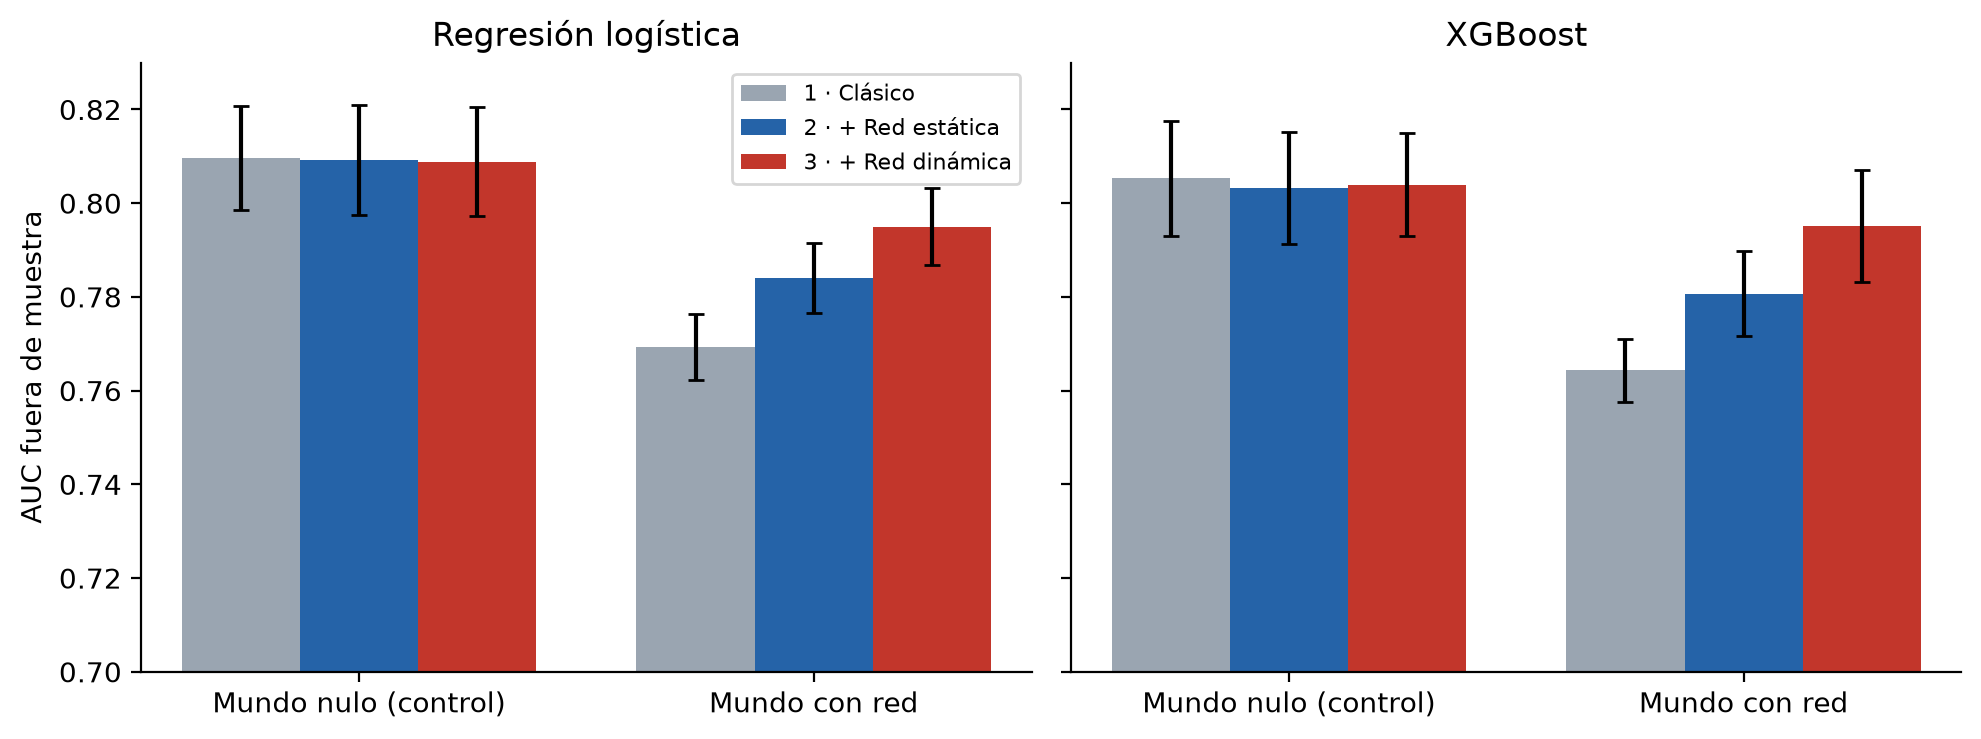
\includegraphics[width=\textwidth]{tarea6_auc_niveles.png}
\caption{AUC fuera de muestra por nivel de variables. En el mundo nulo los tres
niveles empatan; en el mundo con red cada nivel agrega información.}
\end{figure}

\begin{center}
\begin{tabular}{llccc}
\toprule
Mundo & Modelo & 1 · Clásico & 2 · + Red estática & 3 · + Red dinámica \\
\midrule
Nulo (control) & logística & 0.810 & 0.809 & 0.809 \\
Nulo (control) & XGBoost & 0.805 & 0.803 & 0.804 \\
Con red & logística & 0.769 & 0.784 & \textbf{0.795} \\
Con red & XGBoost & 0.764 & 0.781 & \textbf{0.795} \\
\bottomrule
\end{tabular}
\end{center}

\begin{figure}[h]
\centering
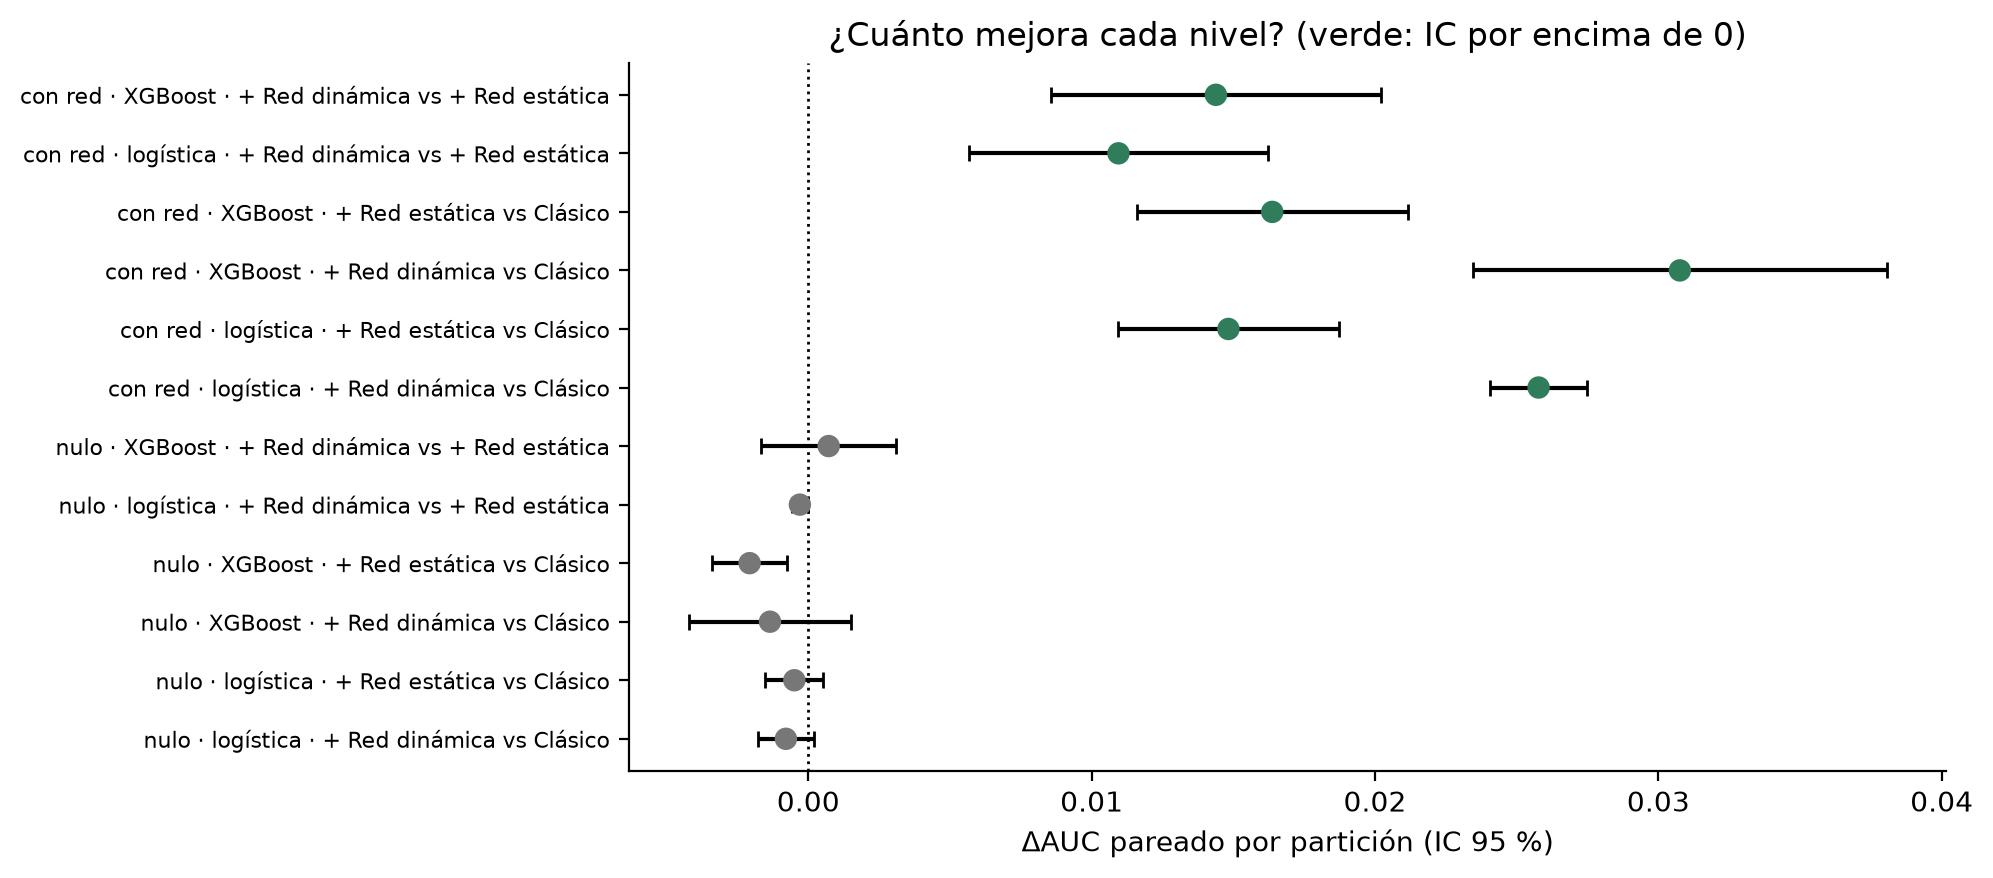
\includegraphics[width=0.92\textwidth]{tarea6_mejoras.png}
\caption{Mejoras pareadas de AUC con su intervalo de confianza del 95~\%. En verde, las
que están claramente por encima de cero.}
\end{figure}

\begin{clave}
En el mundo con red, la \textbf{dinámica mejora sobre la red estática}:
$\Delta\mathrm{AUC}=+0.011$ $[+0.006,+0.016]$ con logística y $+0.014$ $[+0.009,+0.020]$
con XGBoost, positiva en las 5 de 5 particiones; el PR-AUC sube de 0.277 (clásico) a
0.323. Frente al score clásico, el modelo completo gana $+0.026$ a $+0.031$. En el
\textbf{mundo nulo}, las mismas variables no aportan nada ($\Delta\mathrm{AUC}$ entre
$-0.002$ y $+0.001$): la mejora no es un artefacto ni una fuga.
\end{clave}

\section{Sincronización e impago}
\begin{figure}[h]
\centering
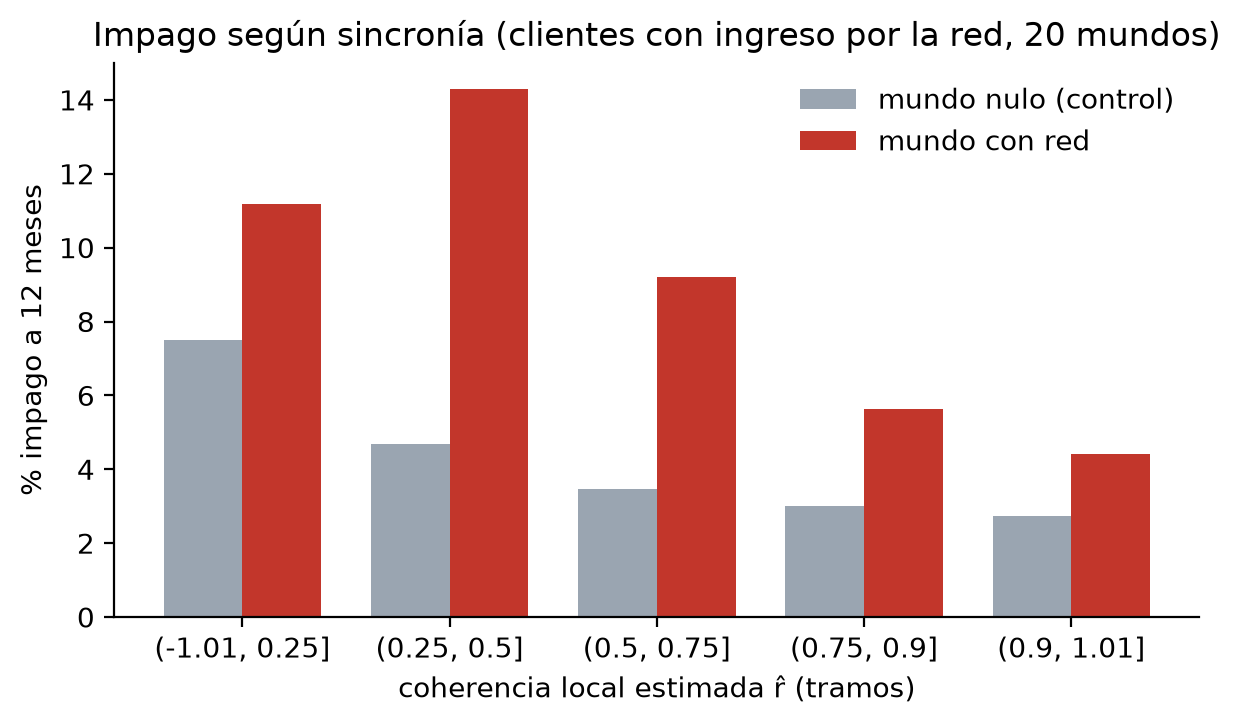
\includegraphics[width=0.8\textwidth]{tarea6_impago_por_r.png}
\caption{Tasa de impago por tramos de coherencia local estimada (solo clientes con
ingreso por la red). Con red, el impago pasa de 4.4~\% (bien sincronizados) a
11–14~\% (desincronizados).}
\end{figure}
\begin{nota}
En el mundo nulo también hay un gradiente (de 2.7~\% a 7.5~\%), pero se explica por
variables clásicas: los informales son más riesgosos y, a la vez, están menos
sincronizados. Por eso esta gráfica, sola, no prueba nada; la prueba es la
comparación de modelos con el control nulo.
\end{nota}

\section{Quiebra de un empleador}
\begin{figure}[h]
\centering
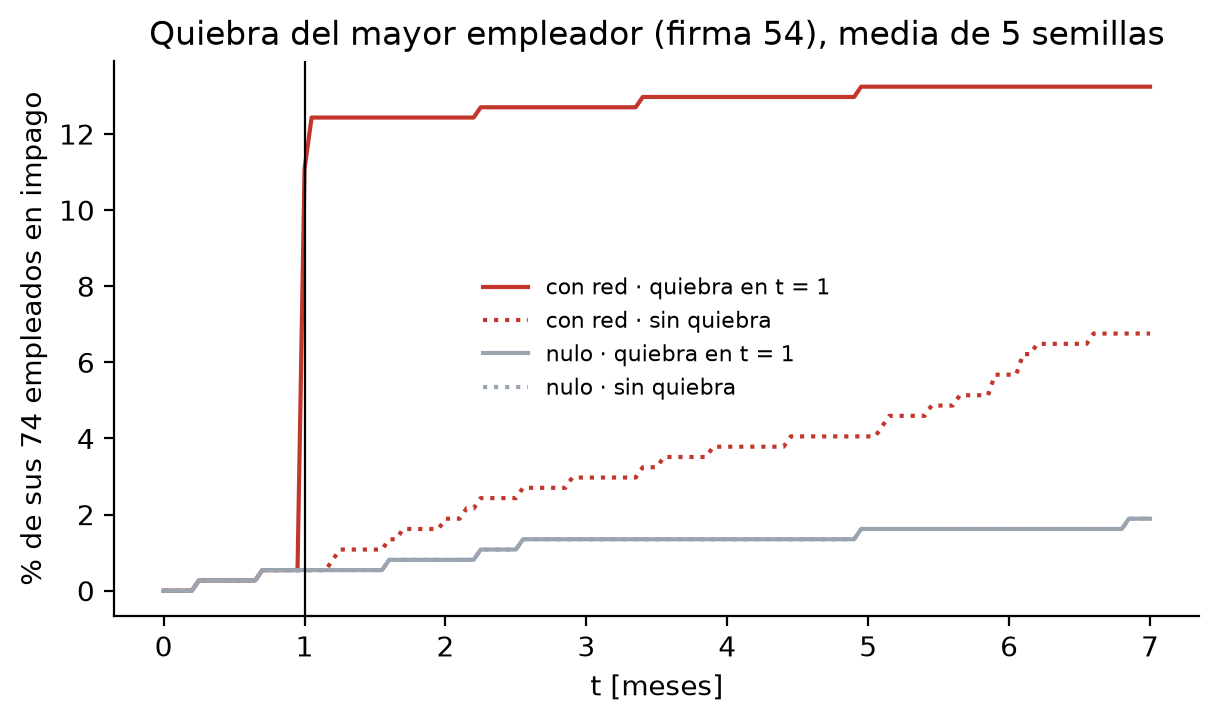
\includegraphics[width=0.8\textwidth]{tarea6_quiebra.png}
\caption{Empleados de la mayor firma de una cartera completa. Con red, la quiebra hace
caer al $\sim$12~\% de inmediato (contra $\sim$1~\% sin quiebra) y a los 6 meses llega a
13~\% (contra 7~\% sin quiebra, por la sola desincronización). En el mundo nulo la quiebra no cambia nada: la curva con y sin quiebra
coinciden.}
\end{figure}

\section{Interpretación y alcance}
\begin{itemize}
\item \textbf{Significa} que, si el mecanismo existe (los ingresos desfasados
generan estrés), entonces es \emph{detectable} solo con el registro de transacciones
que ya tiene un banco, y que aporta algo que la red estática no da.
\item \textbf{Significa} que el diseño experimental distingue señal de fuga: el
control nulo da cero.
\item \textbf{No significa} que el mecanismo exista en la realidad ni que la mejora
real sea de $+0.011$: los números dependen de parámetros ilustrativos ($\gamma$,
$K_\ell$, $\beta_\ell$\ldots).
\item \textbf{Siguiente paso} para convertirlo en evidencia: correr el mismo pipeline
(estimación, variables, evaluación) sobre datos reales anonimizados de una cartera.
El código ya está preparado: no usa nada que un banco no tenga.
\end{itemize}

\part{Montaje del software}
% ===================================================================== PARTE IV
\chapter{Herramientas de software}

\begin{longtable}{p{0.2\textwidth}p{0.74\textwidth}}
\toprule
\textbf{Herramienta} & \textbf{Qué es y para qué se usa aquí} \\
\midrule
\endhead
Python 3.12 & El lenguaje del proyecto. Las librerías científicas hacen el trabajo
pesado: \textbf{NumPy} (vectores y matrices), \textbf{SciPy} (valores propios, matrices
dispersas, estadística), \textbf{pandas} (tablas), \textbf{NetworkX} (grafos),
\textbf{scikit-learn} y \textbf{XGBoost} (aprendizaje automático), \textbf{PyTorch} y
\textbf{PyTorch Geometric} (GCN y PINN), \textbf{SHAP} (explicaciones),
\textbf{Plotly} y \textbf{Matplotlib} (gráficas). \\
uv & Gestor de entornos y dependencias (como \texttt{pip} + \texttt{venv}, más rápido).
\texttt{uv sync} instala exactamente las versiones de \texttt{uv.lock}; \texttt{uv run}
ejecuta dentro de ese entorno. \\
\texttt{pyproject.toml} & Ficha del proyecto: nombre, versión, dependencias, comando
\texttt{pulso} y configuración de las herramientas. \\
YAML & Formato de texto para configuración (como un diccionario de Python en un
archivo). Cada experimento queda documentado con sus parámetros exactos. \\
Parquet & Formato de tabla en archivo: como CSV, pero comprimido, rápido y con tipos
fijos. \texttt{pd.read\_parquet} lo lee. \\
pytest & Corre las pruebas: funciones \texttt{test\_...} que verifican resultados. \\
ruff & Revisa el estilo y errores comunes sin ejecutar el código, y lo formatea. \\
git & Historial de versiones. Cada fase se trabajó en una \emph{rama} y se unió a
\texttt{main} solo con las pruebas en verde. \\
Streamlit & Convierte scripts de Python en una aplicación web interactiva. \\
Docker & Empaqueta Python, librerías, código, datos y modelos en una \emph{imagen} que
corre igual en cualquier computador. \\
GitHub Actions & Integración continua: en cada cambio subido corre ruff, pytest y
construye la imagen Docker. \\
LaTeX & Con el que se escribió esta guía y la presentación. \\
\bottomrule
\end{longtable}

% ---------------------------------------------------------------------------
\chapter{Instalación y ejecución}

\section{Instalación}
\begin{enumerate}
\item Instalar \texttt{uv} (\url{https://docs.astral.sh/uv/}).
\item En la carpeta del proyecto:
\begin{codigo}[label=terminal]
uv sync                      # crea el entorno e instala todo
uv run pytest -m "not slow"  # pruebas rápidas (~10 s)
uv run pytest                # todas las pruebas (~1 min)
\end{codigo}
\end{enumerate}

\section{La aplicación}
\begin{codigo}[label=terminal]
uv run streamlit run app/Inicio.py      # abre http://localhost:8501
\end{codigo}
Si el puerto 8501 está ocupado: \texttt{--server.port=8502}.

\section{Comandos del proyecto}
\begin{codigo}[label=terminal]
uv run pulso sweep  configs/sweep.yaml    # dataset de la tarea 5 (~20 min, 8 núcleos)
uv run pulso train  configs/train.yaml    # modelos de la tarea 5
uv run pulso world  configs/world.yaml    # un mundo multicapa -> data/world/demo
uv run pulso credit configs/credit.yaml   # experimento y modelos de la tarea 6 (~20 s)
uv run pulso --help                       # ayuda
\end{codigo}

\section{Con Docker}
\begin{codigo}[label=terminal]
docker build -t pulso .
docker run -p 8501:8501 pulso
\end{codigo}
La imagen incluye los datos y modelos ya entrenados: la app funciona sin correr
ningún experimento.

\section{Regenerar esta documentación}
\begin{codigo}[label=terminal]
PYTHONPATH=src uv run python docs/latex/figuras.py   # figuras de la tarea 6
bash docs/latex/compilar.sh                          # todos los PDF -> docs/Presentaciones/
\end{codigo}

\section{Modificación de parámetros}
Ejemplo: evaluar un acoplamiento de nómina más intenso. Se edita
\archivo{configs/credit.yaml}:
\begin{codigo}[label=configs/credit.yaml]
dynamics:
  alpha: 1.0                       # 1/mes: el déficit se corrige en ~1 mes
  beta: {N: 0.5, S: 0.4, T: 0.3}   # amplificación del déficit de quien paga
  K: {N: 0.8, S: 1.0, T: 0.3}      # ajuste del ritmo al de los pagadores
  gamma: 0.5                       # ingreso desfasado que se vuelve déficit
  loss: 1.0                        # perder un pagador del 100 % del ingreso
  noise: 0.3                       # choques idiosincráticos de liquidez
\end{codigo}
y se vuelve a correr \texttt{uv run pulso credit configs/credit.yaml}. No se toca el
código.

% ---------------------------------------------------------------------------
\chapter{La aplicación web}

\begin{figure}[h]
\centering
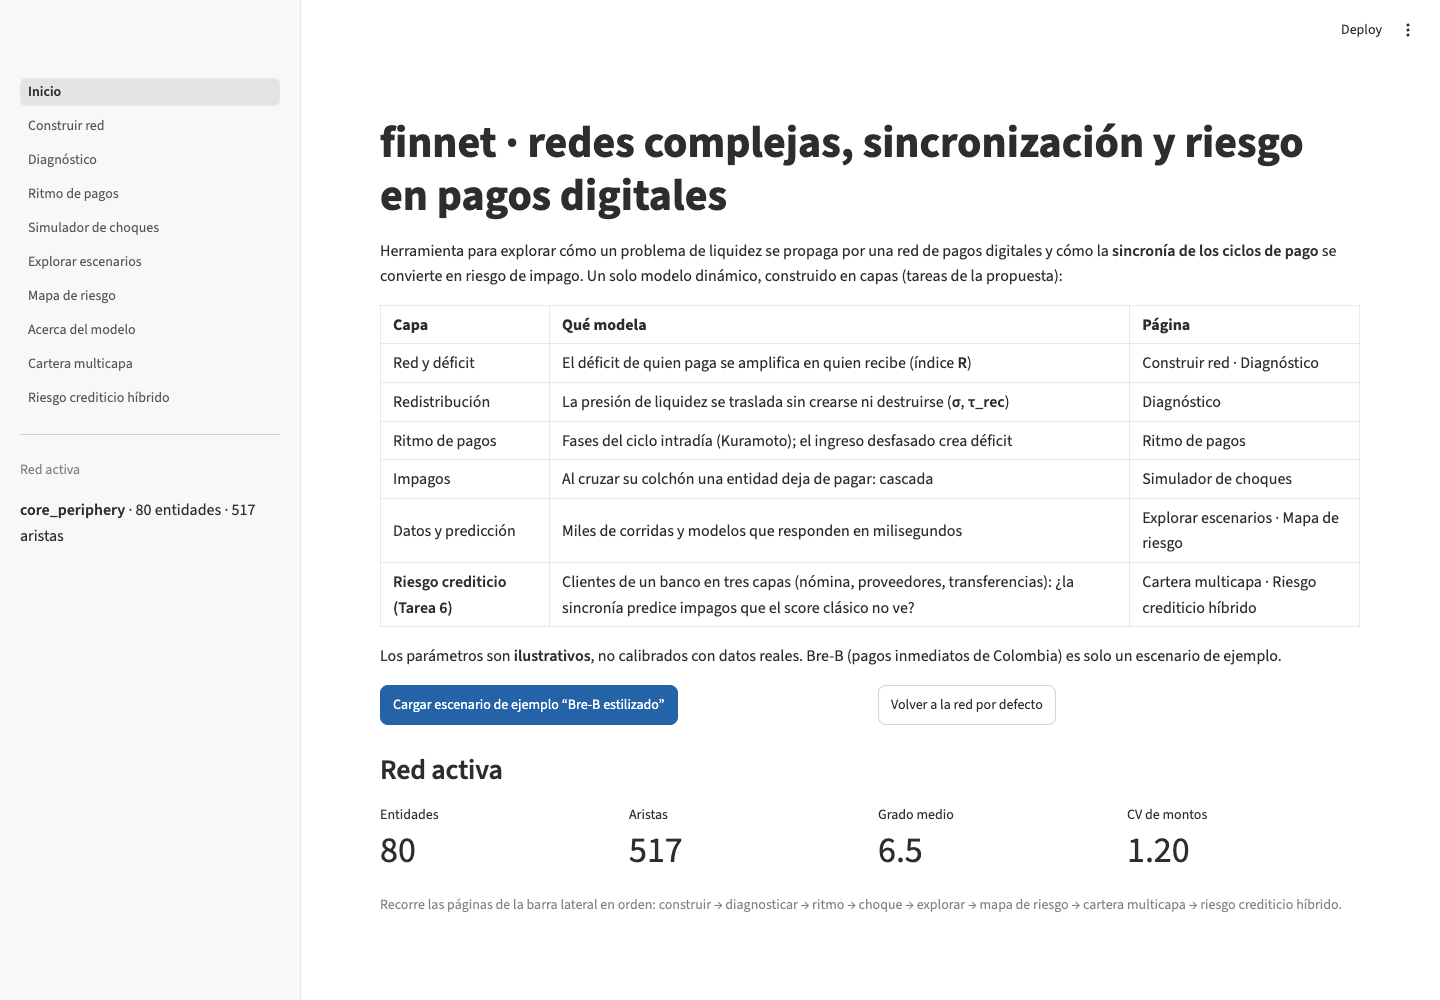
\includegraphics[width=0.92\textwidth]{app_inicio.png}
\caption{Inicio: el resumen de las capas del modelo y la red activa. El botón carga el
escenario de ejemplo ``Bre-B estilizado'' (núcleo-periferia, 245 entidades).}
\end{figure}

\begin{description}
\item[Construir red.] Se elige topología, tamaño, grado medio y dispersión de montos.
\item[Diagnóstico.] $R$, estabilidad $\sigma$ con semáforo, tiempo de recuperación,
$\lambda_2$, comunidades y ranking de entidades por importancia y vulnerabilidad.
\item[Ritmo de pagos.] $K$, dispersión de ritmos, $\gamma$; círculo de fases animado,
$r(t)$ y déficit; se puede desconectar una entidad a mitad de la corrida.
\item[Simulador de choques.] Se elige entidad y tipo de choque; cascada animada,
porcentaje en impago, liquidez no pagada, DebtRank y línea de tiempo de eventos.
\item[Explorar escenarios.] El dataset de 20\,000 escenarios: dónde colapsa la red.
\item[Mapa de riesgo.] Predicción instantánea por entidad (GCN, XGBoost), explicación
SHAP y botón ``verificar con simulación''.
\item[Acerca del modelo.] Ecuaciones, supuestos y límites.
\item[Cartera multicapa.] Tarea 6: la cartera del banco, sus capas, la sincronía
global estimada contra la real, impago según sincronía y el escenario de quiebra de
un empleador.
\item[Riesgo crediticio híbrido.] Tarea 6: la comparación de los tres niveles con su
control, la PD por cliente (clásica contra híbrida), los clientes con ``riesgo
oculto'' y la explicación SHAP de cada predicción.
\end{description}

\begin{figure}[p]
\centering
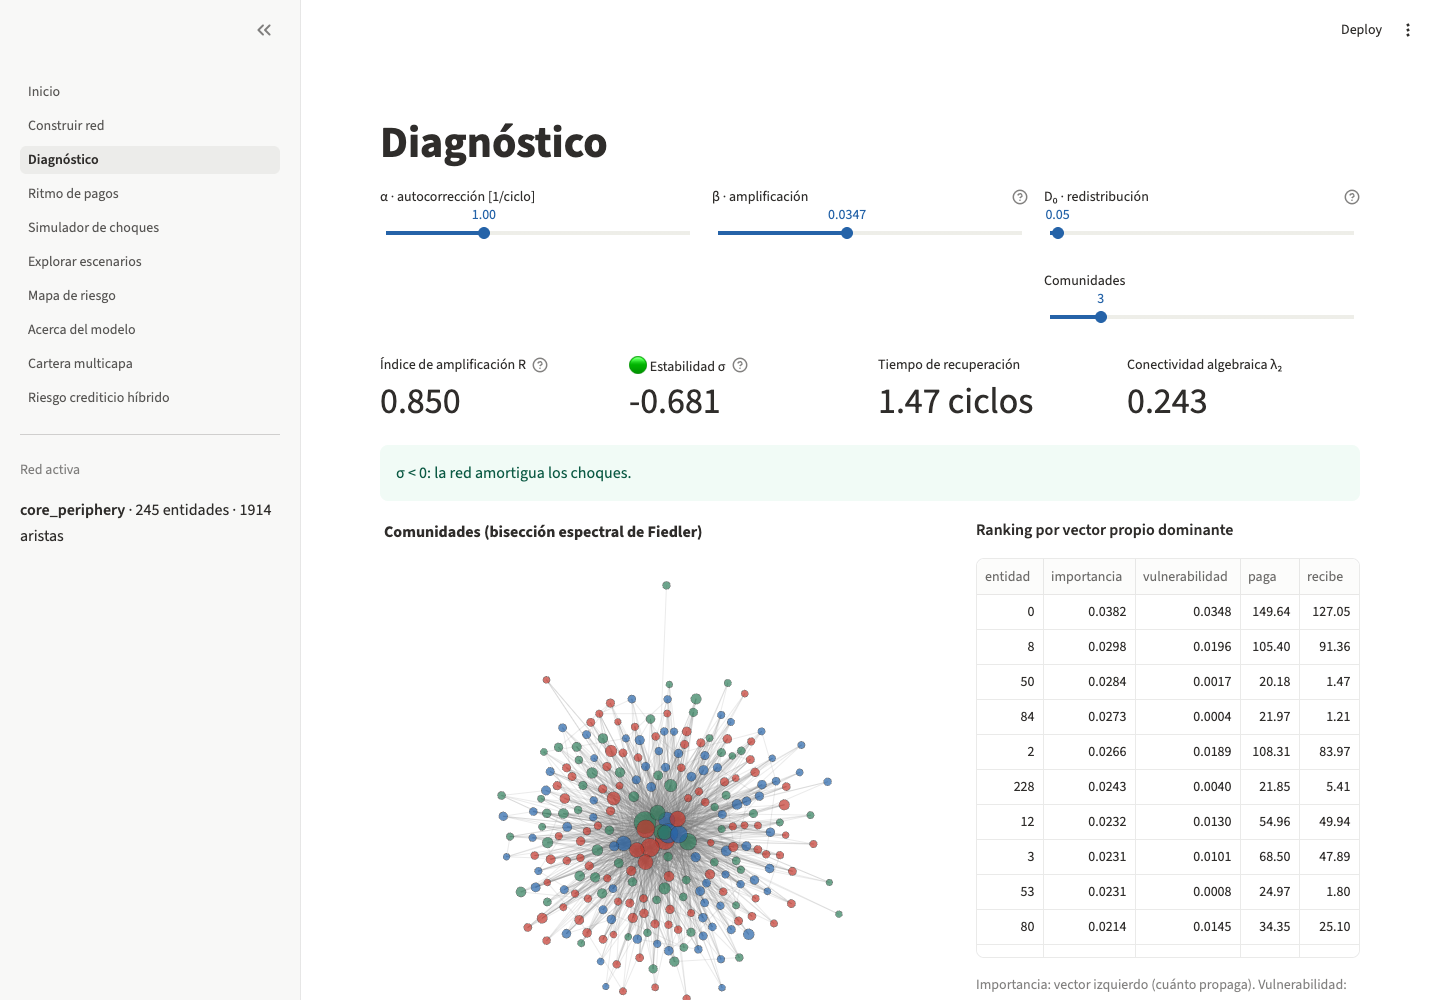
\includegraphics[width=0.49\textwidth]{app_diagnostico.png}\hfill
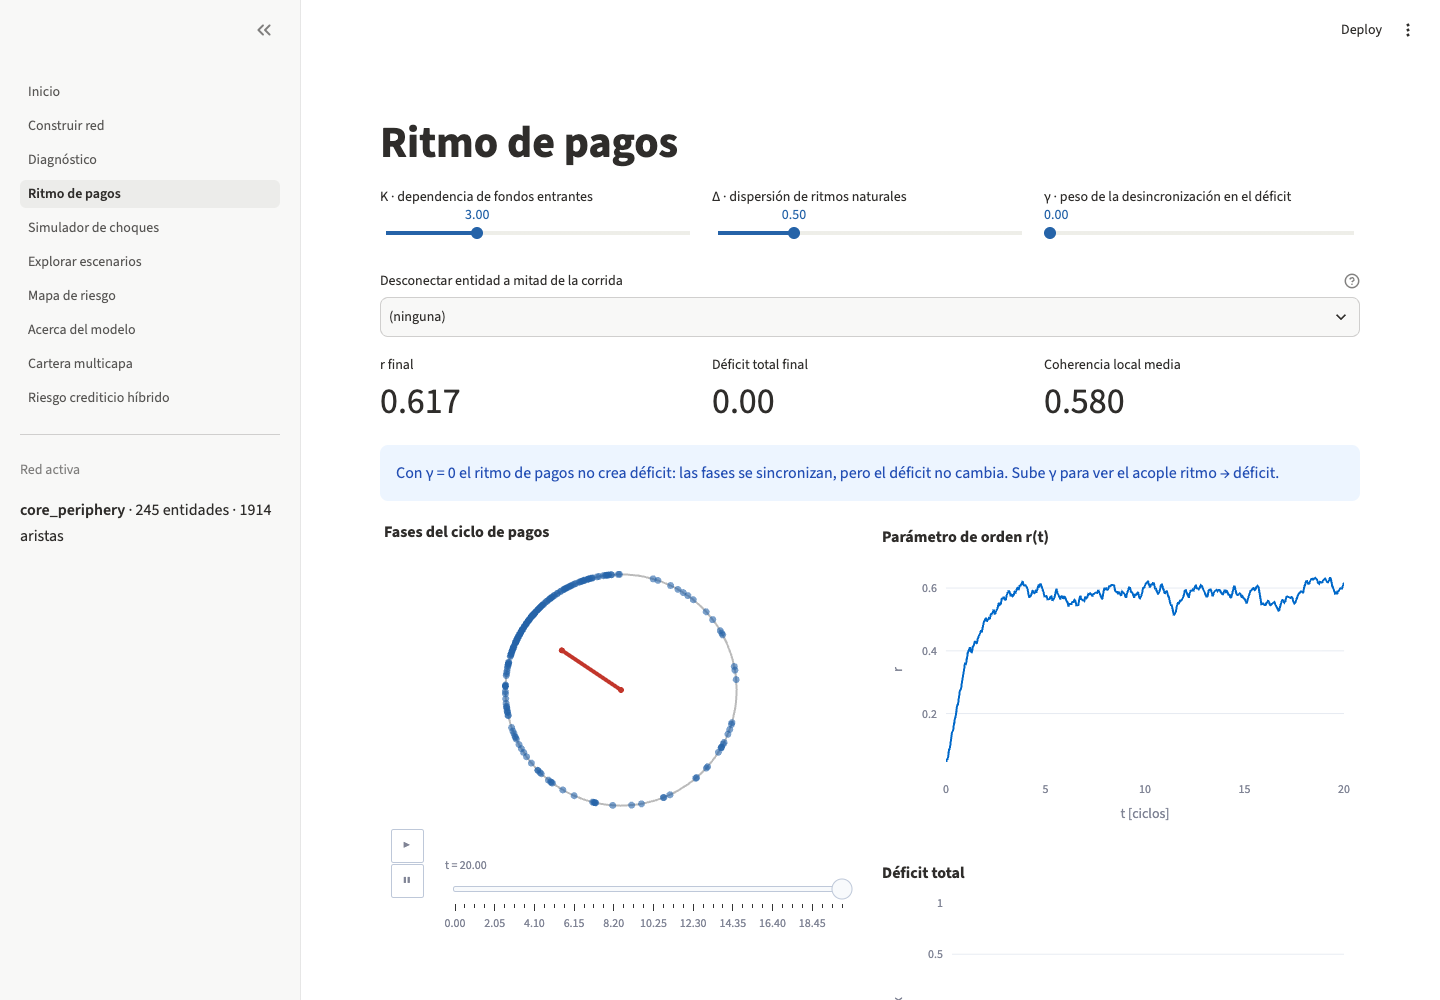
\includegraphics[width=0.49\textwidth]{app_ritmo.png}\\[4pt]
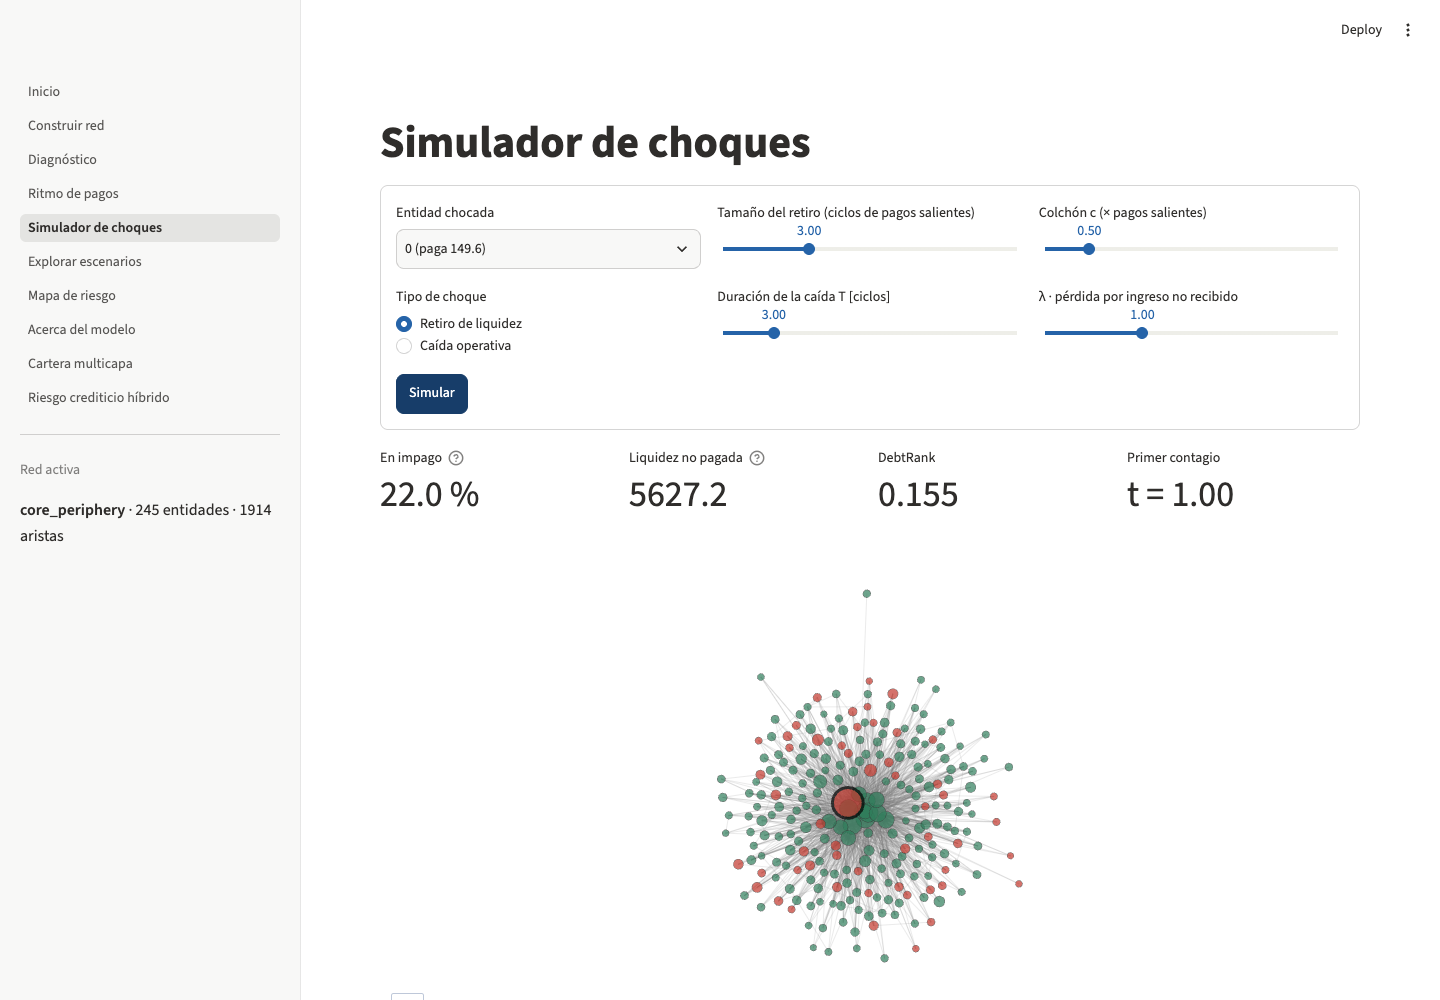
\includegraphics[width=0.49\textwidth]{app_simulador.png}\hfill
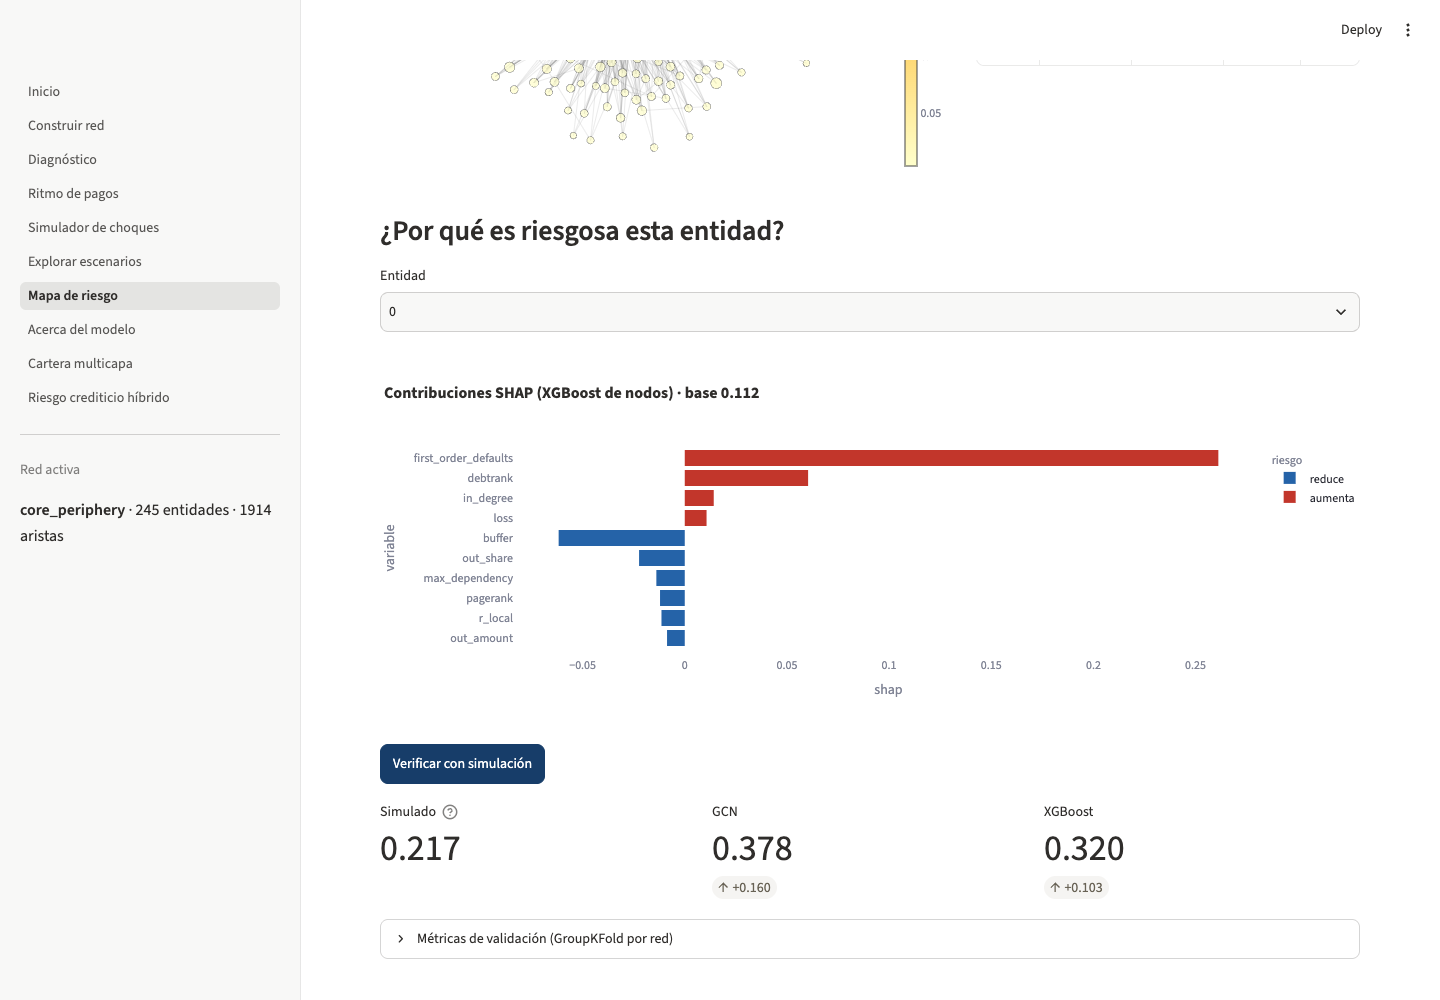
\includegraphics[width=0.49\textwidth]{app_mapa.png}
\caption{Diagnóstico, Ritmo de pagos, Simulador de choques y Mapa de riesgo.}
\end{figure}

\begin{figure}[p]
\centering
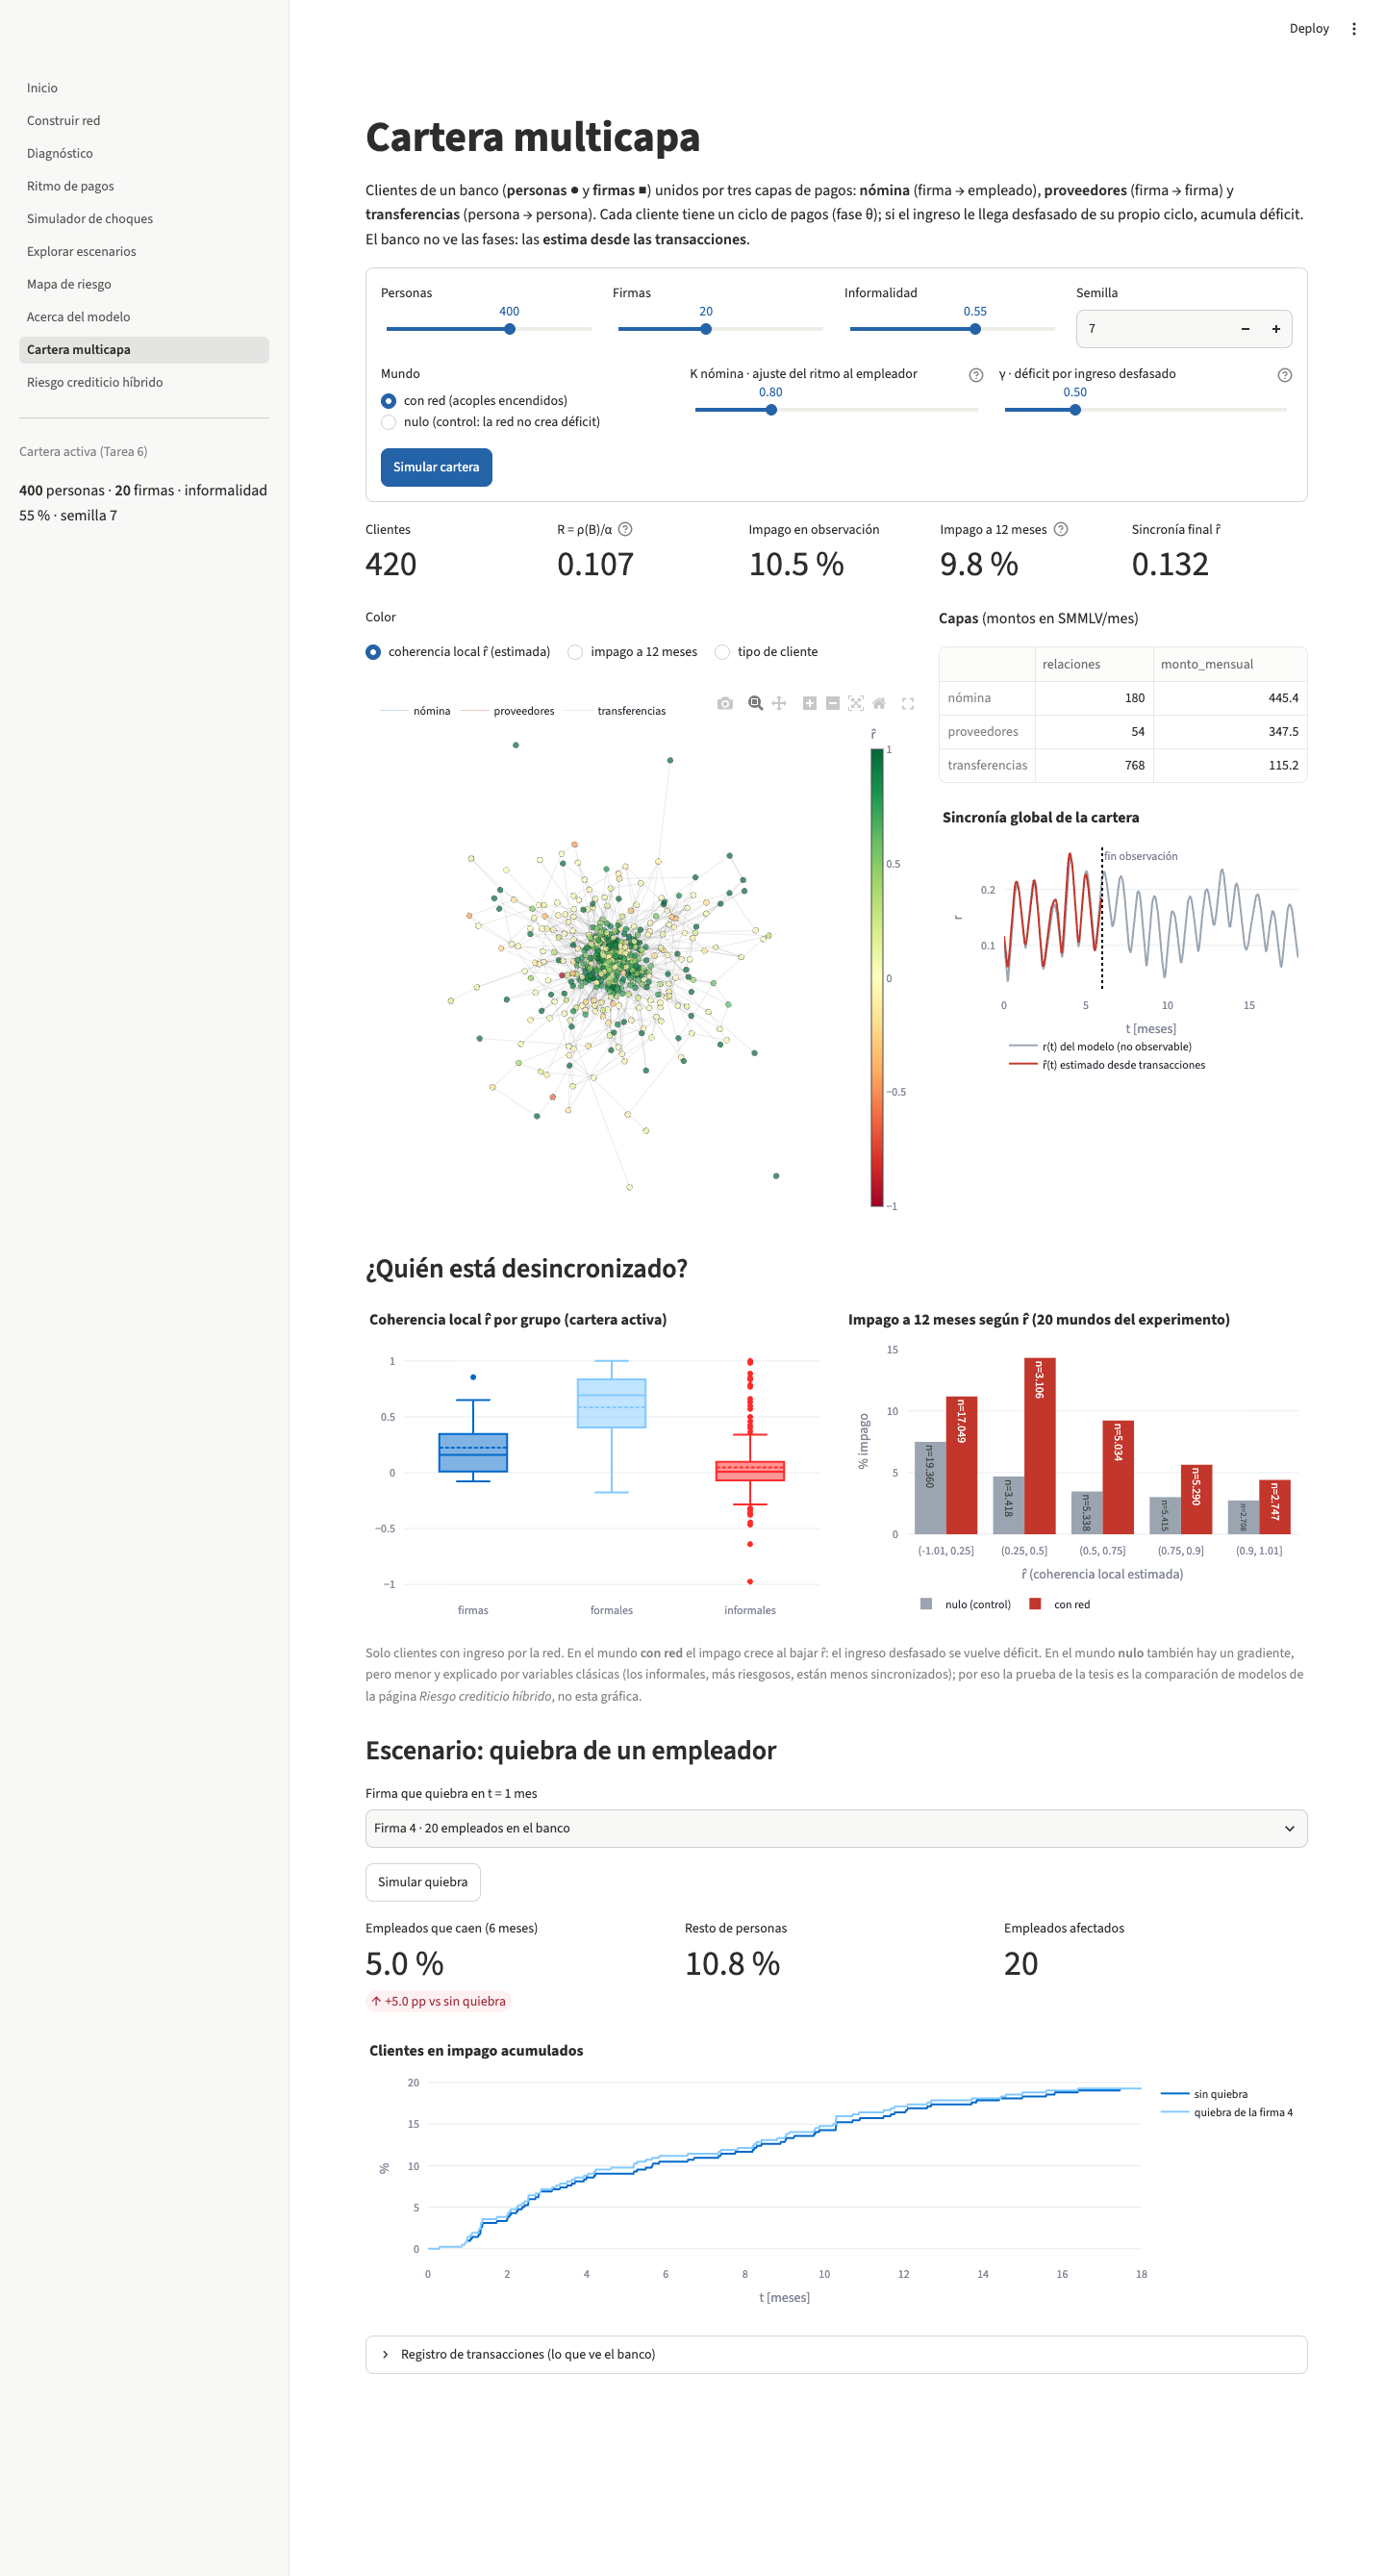
\includegraphics[height=0.86\textheight]{app_cartera_completa.png}
\caption{Cartera multicapa, con el escenario de quiebra simulado.}
\end{figure}

\begin{figure}[p]
\centering
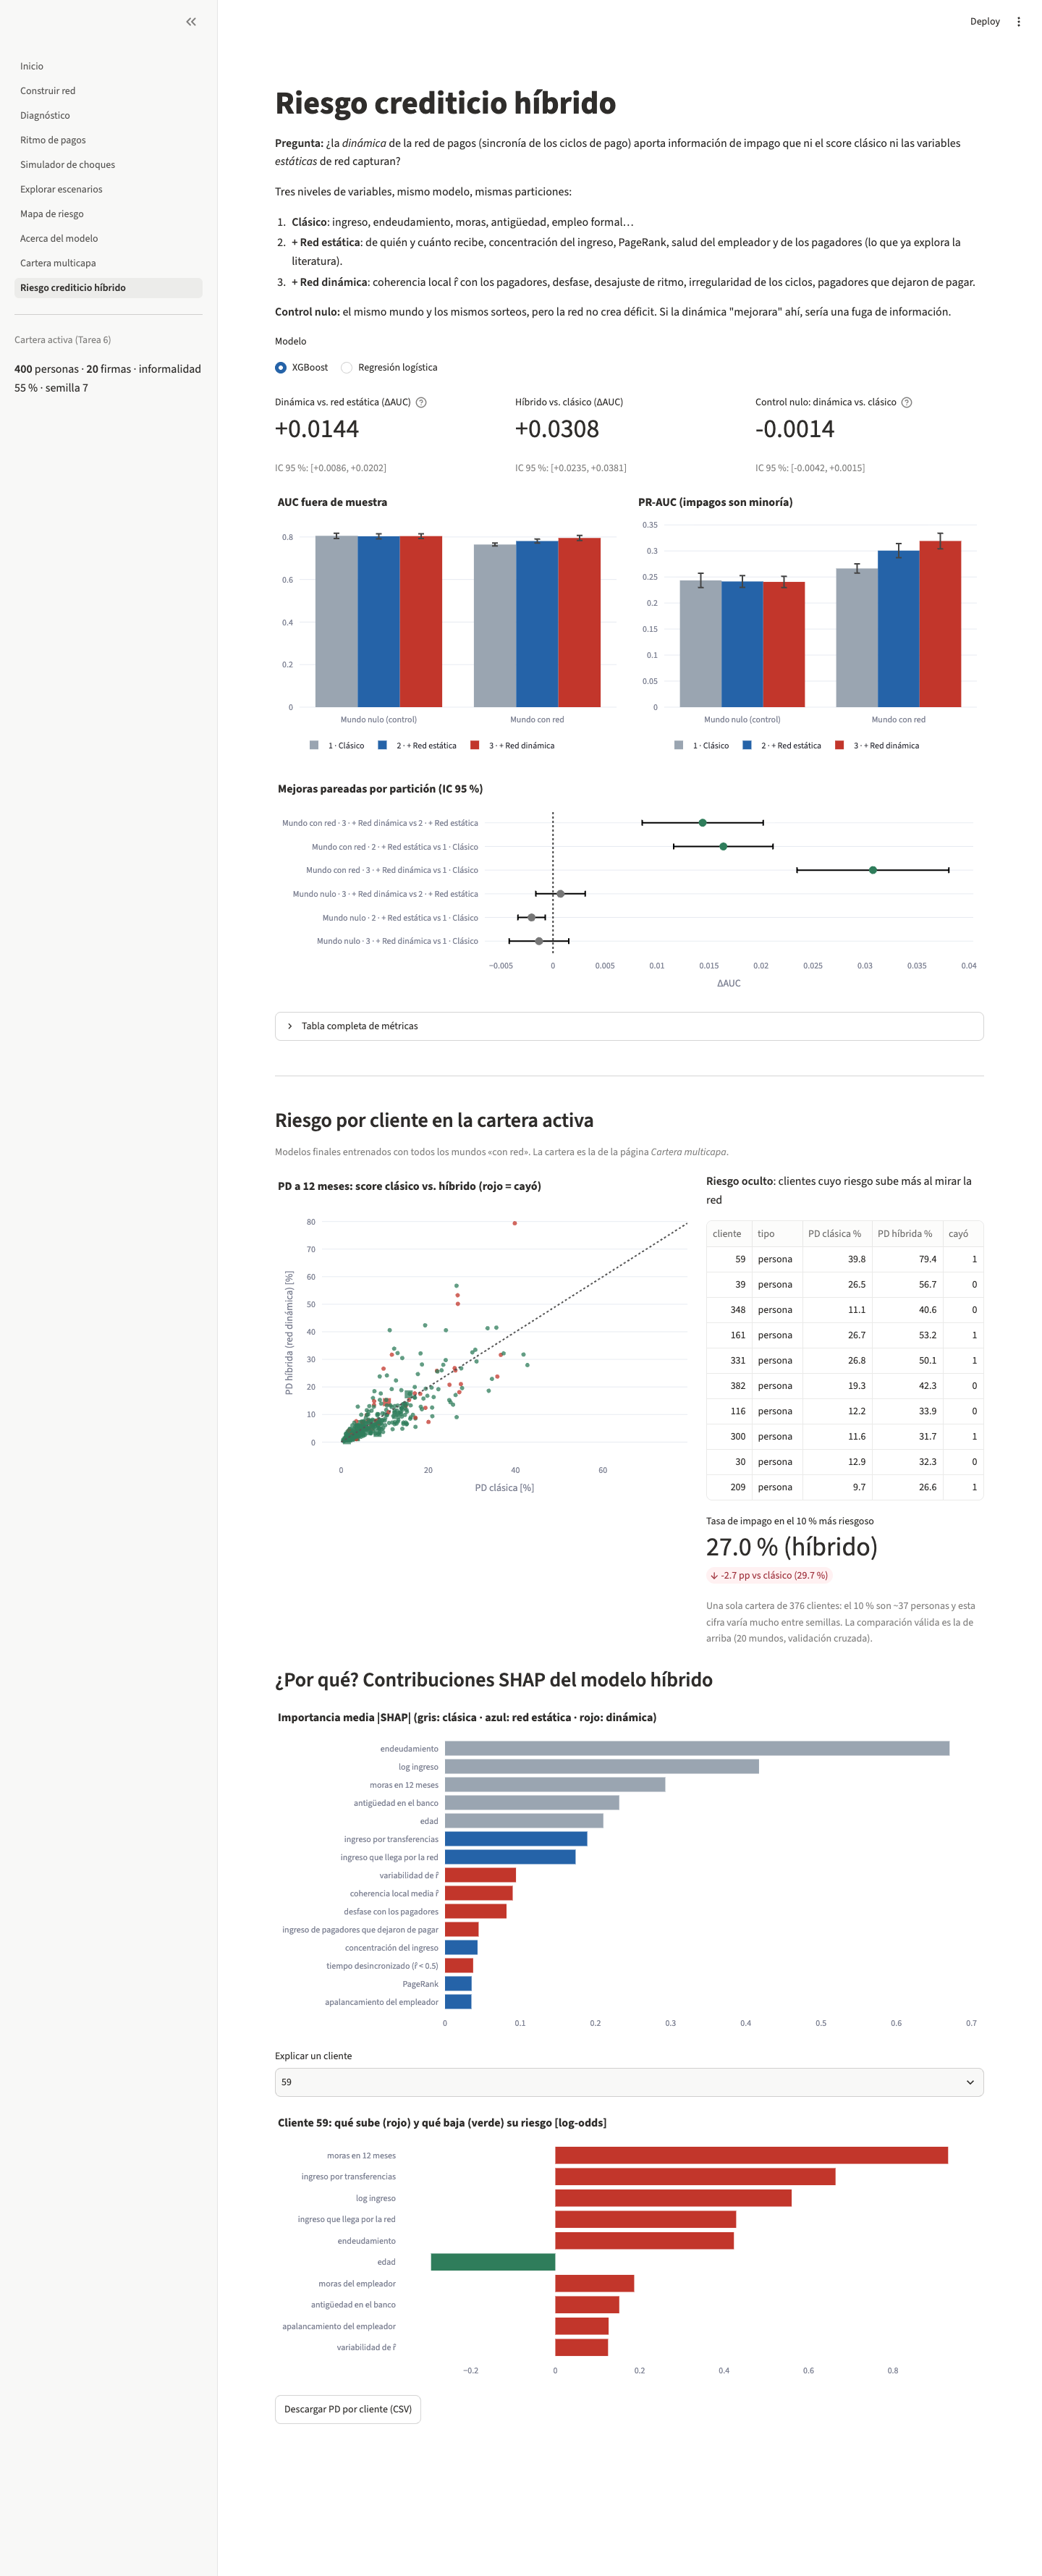
\includegraphics[height=0.86\textheight]{app_hibrido_completa.png}
\caption{Riesgo crediticio híbrido.}
\end{figure}

% ---------------------------------------------------------------------------
\chapter{Organización del proyecto}

\begin{codigo}[label=estructura de carpetas]
pulso/
├── README.md, CHANGELOG.md        qué es, cómo usarlo, historial de versiones
├── pyproject.toml, uv.lock        dependencias exactas
├── Dockerfile, .dockerignore      imagen de la app
├── .github/workflows/ci.yml       pruebas y Docker en cada cambio
├── configs/                       TODOS los parámetros (YAML)
│   ├── default.yaml, breb_example.yaml       app, tareas 1–4
│   ├── sweep.yaml, train.yaml, pinn.yaml     tarea 5
│   └── world.yaml, credit.yaml               tarea 6
├── src/pulso/                    el núcleo (paquete de Python)
│   ├── networks, model, integrate, spectral, cascades, metrics
│   ├── experiments, ml/            tarea 5
│   ├── world/, credit/             tarea 6
│   ├── service.py, schema.py, config.py, cli.py, viz.py
├── app/                           Inicio.py, common.py, pages/1..9
├── tests/                         test_fase1..6, test_fase10..12, test_app
├── notebooks/                     01..06: exploración y figuras por tarea
├── data/                          datasets (tarea 5) y data/credit/ (tarea 6)
├── models/                        modelos versionados; models/credit/v1
├── figures/                       figuras de las tareas 1–6
└── docs/
    ├── Presentaciones/
    │   ├── v1/                    esta guía y la presentación completa
    │   └── v2/                    presentación breve, guion y manual de la app
    ├── bibliografia.md
    ├── diseno/                    especificación de diseño de la tarea 6
    └── latex/                     fuentes de los PDF, figuras y compilar.sh
\end{codigo}

Archivos que \emph{no} se guardan en git porque se regeneran: el entorno
(\texttt{.venv/}), las cachés (\texttt{\_\_pycache\_\_}, \texttt{.pytest\_cache},
\texttt{.ruff\_cache}), los temporales (\texttt{data/tmp/}) y la tabla grande de
clientes de la tarea 6 (\texttt{data/credit/clientes.parquet}, se rehace en segundos).

% ---------------------------------------------------------------------------
\chapter{Problemas conocidos y trabajo futuro}

\section{Problemas conocidos (macOS)}
\begin{itemize}
\item \texttt{ModuleNotFoundError: No module named 'pulso'} dentro de
\texttt{\textasciitilde/Documents}: macOS oculta el archivo \texttt{.pth} de la
instalación editable. Solución: \texttt{chflags -R nohidden .venv}, o anteponer
\texttt{PYTHONPATH=src}.
\item torch y xgboost traen cada uno su propia librería OpenMP; el proyecto carga
xgboost primero y deja torch en un hilo para evitar cierres inesperados.
\end{itemize}

\section{Trabajo futuro}
\begin{enumerate}
\item \textbf{Datos reales}: correr el pipeline de la tarea 6 sobre una cartera
anonimizada. Es el paso que convierte el mecanismo en evidencia.
\item \textbf{Revisión bibliográfica sistemática} (Scopus, Web of Science) sobre
sincronización y riesgo de crédito.
\item \textbf{Fecha de cuota y plazos} como forzamiento externo del ritmo.
\item \textbf{Retroalimentación}: que el déficit también cambie el ritmo de pago.
\item \textbf{Observabilidad parcial}: un banco solo ve a sus clientes; el operador de
un sistema interoperable como Bre-B ve la red completa.
\end{enumerate}

\appendix
\chapter{Glosario}
\label{ap:glosario}
\begin{description}[style=nextline,leftmargin=0.5cm]
\item[AUC (ROC-AUC)] Probabilidad de que el modelo califique a un caso positivo (cae)
por encima de uno negativo. 0.5 es azar; 1 es perfecto.
\item[Brier] Error cuadrático medio de una probabilidad predicha. Menor es mejor.
\item[Calibración] Que las probabilidades predichas coincidan con las frecuencias
observadas.
\item[Cascada] Secuencia de impagos donde cada uno provoca otros.
\item[Choque] Evento externo que golpea a una entidad (retiro de liquidez, caída
operativa, quiebra).
\item[Coherencia local $r_i$] Qué tan en fase le llega el ingreso a una entidad
respecto a su propio ciclo ($1$: en fase; $-1$: en contrafase).
\item[Colchón (umbral)] Déficit máximo que una entidad soporta antes del impago.
\item[Control nulo] Mismo experimento con el mecanismo apagado; si el efecto aparece
ahí, es un artefacto.
\item[Déficit] Liquidez que falta para cubrir los pagos del momento.
\item[Dispersa (matriz)] Matriz que solo guarda los valores distintos de cero.
\item[Fase $\theta$] Posición dentro del ciclo de pagos, como la aguja de un reloj.
\item[Fuga de información] Cuando el modelo usa, sin querer, datos que no tendría en
la realidad; infla los resultados.
\item[GroupKFold] Validación cruzada que nunca pone el mismo grupo (red o mundo) en
entrenamiento y prueba a la vez.
\item[Impago] No pagar lo que se debía.
\item[Índice de amplificación $R$] $\beta\rho(W)/\alpha$: menor que 1, la red
amortigua; mayor que 1, amplifica.
\item[Informalidad] Trabajo sin empleador formal; aquí, personas sin capa de nómina.
\item[Kuramoto] Modelo de osciladores acoplados que explica la sincronización.
\item[Laplaciano] Matriz que describe la difusión en una red; conserva el total.
\item[Liquidez] Dinero disponible en el momento en que se necesita.
\item[Parquet] Formato de archivo para tablas.
\item[PD] Probabilidad de impago (\emph{probability of default}).
\item[Radio espectral $\rho(W)$] El mayor valor propio de $W$.
\item[RK4] Método de Runge–Kutta de orden 4 para integrar ecuaciones diferenciales.
\item[Riesgo crediticio] Riesgo de que un deudor no pague su crédito.
\item[Riesgo sistémico] Riesgo de que fallas locales se propaguen a todo el sistema.
\item[Score crediticio] Modelo que estima la PD a partir de variables del cliente.
\item[Semilla] Número que fija el azar: misma semilla, mismo resultado.
\item[SHAP] Método que reparte una predicción entre las variables que la causan.
\item[Solvencia] Tener más activos que deudas en total.
\item[Verdad del terreno] Valores reales (aquí, simulados) que sirven para evaluar
pero que ningún modelo puede ver.
\item[XGBoost] Modelo de muchos árboles de decisión que se corrigen unos a otros.
\item[YAML] Formato de texto para configuraciones.
\end{description}

\chapter{Referencias}
\begin{itemize}[leftmargin=*]
\item Acebrón, J. A., et al. (2005). The Kuramoto model. \emph{Rev. Mod. Phys.} 77, 137.
\item Acemoglu, D., Ozdaglar, A., \& Tahbaz-Salehi, A. (2015). Systemic risk and
stability in financial networks. \emph{American Economic Review} 105(2).
\item Allen, F., \& Gale, D. (2000). Financial contagion. \emph{J. Political Economy} 108(1).
\item Arenas, A., et al. (2008). Synchronization in complex networks. \emph{Physics Reports} 469.
\item Barabási, A.-L. (2016). \emph{Network Science}. Cambridge University Press.
\item Barabási, A.-L., \& Albert, R. (1999). Emergence of scaling in random networks.
\emph{Science} 286.
\item Battiston, S., et al. (2012). DebtRank: Too central to fail? \emph{Scientific Reports} 2.
\item Battiston, S., et al. (2007). Credit chains and bankruptcy propagation in
production networks. \emph{J. Econ. Dyn. Control} 31(6).
\item Boccaletti, S., et al. (2006). Complex networks: structure and dynamics.
\emph{Physics Reports} 424.
\item Boccaletti, S., et al. (2014). The structure and dynamics of multilayer
networks. \emph{Physics Reports} 544.
\item Chung, F. (1997). \emph{Spectral Graph Theory}. AMS.
\item Eisenberg, L., \& Noe, T. H. (2001). Systemic risk in financial systems.
\emph{Management Science} 47(2).
\item Gai, P., \& Kapadia, S. (2010). Contagion in financial networks. \emph{Proc. R. Soc. A} 466.
\item Goodfellow, I., Bengio, Y., \& Courville, A. (2016). \emph{Deep Learning}. MIT Press.
\item Haldane, A. G., \& May, R. M. (2011). Systemic risk in banking ecosystems.
\emph{Nature} 469.
\item Karniadakis, G. E., et al. (2021). Physics-informed machine learning.
\emph{Nature Reviews Physics} 3.
\item Kipf, T. N., \& Welling, M. (2017). Semi-supervised classification with graph
convolutional networks. \emph{ICLR}.
\item Letizia, E., \& Lillo, F. (2019). Corporate payments networks and credit risk
rating. \emph{EPJ Data Science} 8, 21.
\item Merton, R. C. (1974). On the pricing of corporate debt. \emph{J. Finance} 29(2).
\item Newman, M. E. J. (2003). The structure and function of complex networks.
\emph{SIAM Review} 45.
\item Newman, M. E. J. (2010). \emph{Networks: An Introduction}. Oxford University Press.
\item Óskarsdóttir, M., \& Bravo, C. (2021). Multilayer network analysis for improved
credit risk prediction. \emph{Omega} 105.
\item Pikovsky, A., Rosenblum, M., \& Kurths, J. (2001). \emph{Synchronization}.
Cambridge University Press.
\item Raissi, M., Perdikaris, P., \& Karniadakis, G. E. (2019). Physics-informed neural
networks. \emph{J. Comput. Phys.} 378.
\item Rodrigues, F. A., et al. (2016). The Kuramoto model in complex networks.
\emph{Physics Reports} 610.
\item Shi, J., \& Malik, J. (2000). Normalized cuts and image segmentation.
\emph{IEEE TPAMI} 22(8).
\item Tobback, E., et al. (2017). Bankruptcy prediction for SMEs using relational
data. \emph{Decision Support Systems} 102.
\item Watts, D. J. (2002). A simple model of global cascades on random networks.
\emph{PNAS} 99(9).
\item Banco Central do Brasil, Working Papers 551 y 584.
\end{itemize}
\begin{nota}
Las referencias de Tobback et al., Óskarsdóttir y Bravo y Battiston et al.\ (2007) se
citaron de memoria: verifique volumen y páginas antes de usarlas en un documento
formal.
\end{nota}


\end{document}
